\documentclass[12pt, a4paper]{report}
\usepackage[spanish]{babel}
\usepackage[utf8]{inputenc}
\usepackage{graphicx}
\usepackage{amsmath}
\usepackage{amssymb}
\usepackage{hyperref}
\usepackage{geometry}
\usepackage{booktabs}
\usepackage{float}
\usepackage{caption}

% Configuración de geometría
\geometry{
    left=3cm,
    right=2.5cm,
    top=2.5cm,
    bottom=2.5cm
}

% Configuración de hipervínculos
\hypersetup{
    colorlinks=true,
    linkcolor=black,
    filecolor=magenta,      
    urlcolor=blue,
    citecolor=black,
}

\begin{document}

% --- PORTADA ---
\begin{titlepage}
    \centering
    {\Large \textbf{Universidad Yachay Tech} \par}
    \vspace{0.5cm}
    {\large \textbf{Escuela de Ciencias Matemáticas y Computacionales} \par}
    \vspace{0.5cm}
    {\large \textbf{Maestría en Inteligencia Artificial} \par}
    \vspace{2cm}
    
    {\Large \textbf{Título:} \textit{Optimización de Tiempos de Espera en Intersecciones mediante Aprendizaje por Refuerzo Profundo y Simulación} \par}
    \vspace{3cm}
    
    {\large \textbf{Autor:} Bryan Ortega \par}
    \vspace{0.5cm}
    {\large \textbf{Director:} Tito Rolando Armas Andrade \par}
    \vspace{2cm}
    
    {\large \textbf{Fecha:} Noviembre, 2025 \par}
    
    \vfill
\end{titlepage}

% --- RESUMEN ---
\chapter*{Resumen}
\addcontentsline{toc}{chapter}{Resumen}

Este trabajo presenta el desarrollo de un sistema de control semafórico adaptativo basado en \textbf{Deep Reinforcement Learning (DRL)} utilizando el algoritmo \textbf{Proximal Policy Optimization (PPO)} integrado con el simulador microscópico de tráfico \textbf{SUMO}. El objetivo principal es reducir la congestión urbana mediante la optimización dinámica de tiempos semafóricos en una intersección crítica.

El agente aprende a manejar condiciones de tráfico altamente variables gracias a una función de recompensa diseñada para balancear eficiencia y estabilidad, incorporando penalizaciones por colas, desequilibrio direccional y cambios excesivos de fase. El entrenamiento se realizó bajo un perfil de tráfico dinámico de 60 minutos con múltiples picos de demanda.

Los resultados muestran una \textbf{reducción aproximada del 60\% en la longitud promedio de colas} y un \textbf{incremento del 4.5\% en el throughput} respecto a un controlador de tiempo fijo. Estos resultados demuestran la efectividad del enfoque DRL + SUMO para mejorar la movilidad urbana. Finalmente, se discuten las limitaciones actuales y se proponen líneas de trabajo futuro, incluyendo control multiagente y percepción mediante visión por computador.

\vspace{1em}
\noindent \textbf{Palabras clave:} semáforos inteligentes, aprendizaje por refuerzo, PPO, SUMO, tráfico urbano.

% --- ABSTRACT ---
\chapter*{Abstract}
\addcontentsline{toc}{chapter}{Abstract}

This thesis presents the development of an adaptive traffic signal controller based on \textbf{Deep Reinforcement Learning (DRL)} using the \textbf{Proximal Policy Optimization (PPO)} algorithm integrated with the microscopic traffic simulator \textbf{SUMO}. The main objective is to reduce urban congestion by dynamically optimizing signal timings in a high-demand intersection.

The agent learns to manage highly variable traffic conditions through a reward function designed to balance efficiency and stability, incorporating penalties for queue length, directional imbalance, and frequent phase switching. Training was conducted under a dynamic 60-minute traffic profile with several demand peaks.

Results show an \textbf{approximate 60\% reduction in average queue length} and a \textbf{4.5\% increase in throughput} compared to a fixed-time controller. These findings demonstrate the effectiveness of combining DRL and SUMO to improve urban mobility. Limitations and future work directions are discussed, including multi-agent control and perception via computer vision.

\vspace{1em}
\noindent \textbf{Keywords:} intelligent traffic lights, reinforcement learning, PPO, SUMO, urban mobility.

% --- TABLA DE CONTENIDOS ---
\tableofcontents

% --- INTRODUCCIÓN ---
\chapter*{Introducción}
\addcontentsline{toc}{chapter}{Introducción}

\section*{Contexto del problema}
El crecimiento urbano y el aumento del parque automotor han provocado que las intersecciones semaforizadas se conviertan en puntos críticos de congestión. Los semáforos tradicionales, basados en ciclos fijos, no consideran la variabilidad temporal del flujo vehicular ni las diferencias entre direcciones. En ciudades como Ibarra, donde la demanda presenta picos súbitos y asimétricos, los controladores fijos generan colas extensas, tiempos de espera elevados y un uso ineficiente del espacio vial.

\section*{Motivación}
La gestión adaptativa del tráfico representa una oportunidad para reducir de manera significativa la congestión mediante el uso de técnicas modernas de inteligencia artificial. Los avances en \textbf{Deep Reinforcement Learning (DRL)} y la capacidad de simular escenarios realistas con \textbf{SUMO} permiten entrenar agentes capaces de aprender políticas óptimas para la asignación de tiempos semafóricos, respondiendo de forma dinámica a cambios en la demanda. Esta tesis busca aplicar dichas técnicas para mejorar la movilidad urbana en un cruce representativo de la ciudad.

\section*{Planteamiento del problema}
Los sistemas semafóricos de tiempo fijo son ineficientes cuando la demanda vehicular no es uniforme ni estable. En situaciones de alto tráfico, estos sistemas mantienen fases verdes incluso cuando no existen vehículos, mientras otras aproximaciones acumulan colas. El problema a resolver es: \textbf{¿cómo optimizar los tiempos semafóricos de una intersección utilizando DRL para minimizar la formación de colas y mejorar el flujo vehicular bajo condiciones dinámicas y variables?}

\section*{Objetivo general}
Desarrollar un sistema de control semafórico adaptativo basado en \textbf{Proximal Policy Optimization (PPO)}, integrado con SUMO, capaz de reducir colas, mejorar el throughput y adaptarse a variaciones en la demanda vehicular.

\section*{Objetivos específicos}
\begin{itemize}
    \item Diseñar e implementar un entorno de simulación de tráfico en SUMO para un cruce urbano representativo.
    \item Definir y configurar un agente DRL basado en PPO para el control de fases semafóricas.
    \item Construir una función de recompensa que guíe al agente hacia políticas eficientes y estables.
    \item Entrenar el agente bajo diferentes perfiles de tráfico dinámico.
    \item Evaluar el desempeño del agente comparándolo con un controlador de tiempo fijo.
\end{itemize}

\section*{Justificación}
El impacto de la congestión vehicular trasciende la mera incomodidad de los conductores; se manifiesta en pérdidas económicas significativas, incremento en el consumo de combustibles fósiles y un aumento preocupante en las emisiones de gases de efecto invernadero. En ciudades en desarrollo como Ibarra, la infraestructura vial rígida no puede expandirse al mismo ritmo que el parque automotor. Por tanto, la optimización del uso de la infraestructura existente se vuelve imperativa.

Implementar estrategias inteligentes basadas en \textbf{Deep Reinforcement Learning (DRL)} permite transitar de un paradigma reactivo y estático a uno proactivo y dinámico. A diferencia de los sistemas tradicionales que requieren costosas recalibraciones manuales, un agente DRL aprende y evoluciona con el tráfico. Además, la integración con simuladores de código abierto y estandarizados como \textbf{SUMO} garantiza no solo la viabilidad técnica y económica del proyecto, sino también su reproducibilidad y rigor científico, abriendo la puerta a futuras implementaciones en hardware real a bajo costo.

\section*{Alcance y limitaciones}
\textbf{Alcance:}
\begin{itemize}
    \item Se estudia una intersección específica con alto flujo vehicular.
    \item El agente controla únicamente el ciclo semafórico.
    \item Las pruebas se realizan en un entorno simulado.
\end{itemize}

\textbf{Limitaciones:}
\begin{itemize}
    \item No se implementa el sistema en infraestructura real.
    \item El modelo no considera peatones ni transporte público.
    \item La percepción del entorno se basa en datos simulados (no cámaras reales).
\end{itemize}

% --- CAPÍTULO 1 ---
\chapter{Marco Teórico}

\section{Conceptos de Tránsito Vehicular}
El análisis del tráfico vehicular se fundamenta en la teoría del flujo vehicular, la cual describe la interacción entre vehículos, conductores e infraestructura. Las variables macroscópicas fundamentales son:

\textbf{Flujo ($q$):} Se define como la tasa a la cual los vehículos pasan por un punto específico de la vía durante un intervalo de tiempo. Se expresa comúnmente en vehículos por hora (veh/h) \cite{1}, \cite{5}.
\begin{equation}
    q = \frac{N}{T}
\end{equation}
Donde $N$ es el número de vehículos que pasan por el punto y $T$ es el intervalo de tiempo de observación.

\textbf{Densidad ($k$):} Representa el número de vehículos ocupando un segmento de longitud unitaria de la vía en un instante dado. Se expresa en vehículos por kilómetro (veh/km) \cite{5}.

\textbf{Velocidad media espacial ($v_s$):} Es la media armónica de las velocidades de los vehículos que pasan por un punto. La relación fundamental del tráfico establece que \cite{1}:
\begin{equation}
    q = k \cdot v_s
\end{equation}
Donde $q$ es el flujo, $k$ es la densidad y $v_s$ es la velocidad media espacial.

\textbf{Diagrama Fundamental:} Describe la relación no lineal entre flujo y densidad. A medida que la densidad aumenta, el flujo crece hasta alcanzar una capacidad máxima ($q_{max}$), punto tras el cual el flujo colapsa debido a la congestión, entrando en un régimen inestable \cite{5}, \cite{6}.

\textbf{Longitud de Cola:} Métrica crítica para el control semafórico, definida como el número de vehículos detenidos o avanzando a una velocidad inferior a un umbral (e.g., 5 km/h) en una aproximación. Minimizar esta variable es el objetivo principal de la mayoría de los sistemas de control adaptativo \cite{3}, \cite{6}.

\textbf{Fase Semafórica:} Intervalo de tiempo durante el cual un conjunto de movimientos vehiculares (e.g., Norte-Sur) tiene derecho de paso (luz verde), mientras que los movimientos conflictivos se mantienen detenidos (luz roja). Un ciclo semafórico completo se compone de una secuencia ordenada de estas fases \cite{5}.

\section{SUMO: Características y Arquitectura}
\textbf{SUMO (Simulation of Urban MObility)} es una suite de simulación de tráfico microscópico, intermodal y de código abierto, ampliamente utilizada en la investigación de ITS \cite{49}. A diferencia de los modelos macroscópicos que tratan el tráfico como un fluido, SUMO modela cada vehículo como un agente individual con sus propios parámetros físicos y de comportamiento.

\textbf{Modelos de Seguimiento (Car-Following):} SUMO implementa por defecto el modelo de Krauss, una variante estocástica que garantiza una conducción libre de colisiones manteniendo una distancia de seguridad basada en la velocidad del vehículo líder \cite{49}.
\begin{equation}
    v_{safe} = v_l(t) + \frac{g(t) - v_l(t) \tau}{ \frac{\bar{v}}{2b} + \tau }
\end{equation}
Donde $v_{safe}$ es la velocidad segura calculada, $v_l(t)$ es la velocidad del vehículo líder en el tiempo $t$, $g(t)$ es la brecha (gap) con el líder, $\tau$ es el tiempo de reacción del conductor, $b$ es la desaceleración máxima posible y $\bar{v}$ es la velocidad media promedio de los vehículos.

\textbf{TraCI (Traffic Control Interface):} Es el componente crucial para esta investigación. TraCI permite la comunicación bidireccional en tiempo real entre SUMO y un controlador externo (en este caso, el script de Python). Esto permite al agente de RL:
\begin{enumerate}
    \item \textbf{Observar:} Leer estados de sensores simulados (inductivos, cámaras virtuales).
    \item \textbf{Actuar:} Modificar las fases de los semáforos dinámicamente en cada paso de simulación.
\end{enumerate}

\begin{figure}[H]
    \centering
    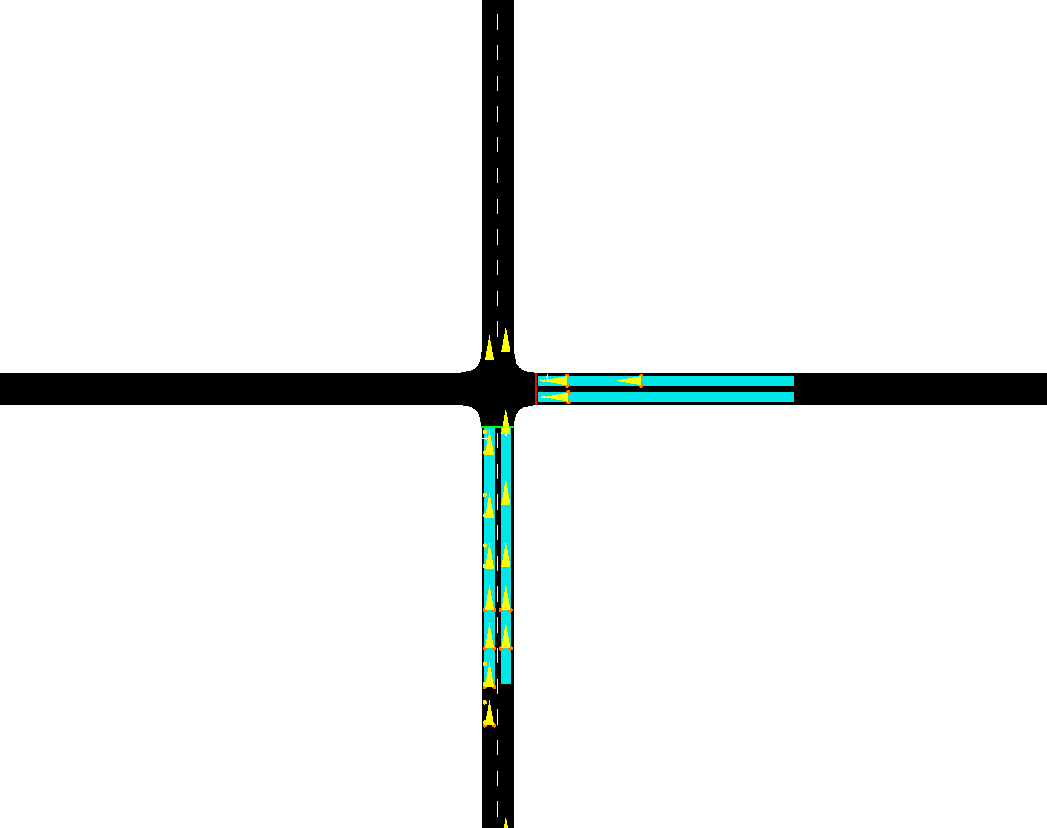
\includegraphics[width=0.8\textwidth]{graficos/Sumo-4vias.png}
    \caption{Visualización de la intersección simulada en SUMO, mostrando las 4 aproximaciones y la gestión semafórica.}
    \label{fig:sumo_4vias}
\end{figure}

\section{Fundamentos de Aprendizaje por Refuerzo (RL)}
El Aprendizaje por Refuerzo es un paradigma de aprendizaje automático donde un agente aprende a tomar decisiones secuenciales interactuando con un entorno. El problema se formaliza matemáticamente como un \textbf{Proceso de Decisión de Markov (MDP)}, definido por la tupla $(S, A, P, R, \gamma)$ \cite{36}:

\begin{itemize}
    \item \textbf{$S$ (Espacio de Estados):} Conjunto de todas las configuraciones posibles del entorno (e.g., posiciones de vehículos, fases actuales).
    \item \textbf{$A$ (Espacio de Acciones):} Conjunto de decisiones disponibles para el agente (e.g., cambiar fase, mantener fase).
    \item \textbf{$P(s'|s,a)$ (Probabilidad de Transición):} Dinámica del entorno que define la probabilidad de pasar al estado $s'$ dado el estado $s$ y la acción $a$.
    \item \textbf{$R(s,a)$ (Función de Recompensa):} Señal escalar que indica la calidad inmediata de la acción tomada.
    \item \textbf{$\gamma \in [0,1]$ (Factor de Descuento):} Determina la importancia de las recompensas futuras frente a las inmediatas.
\end{itemize}

El objetivo del agente es encontrar una política óptima $\pi^*(a|s)$ que maximice el retorno esperado $G_t$, definido como la suma descontada de recompensas futuras:
\begin{equation}
    G_t = \sum_{k=0}^{\infty} \gamma^k R_{t+k+1}
\end{equation}
Donde $G_t$ es el retorno esperado, $\gamma$ es el factor de descuento y $R_{t+k+1}$ es la recompensa recibida en el paso de tiempo $t+k+1$.

\section{Deep Reinforcement Learning y PPO}
El \textbf{Deep Reinforcement Learning (DRL)} integra redes neuronales profundas como aproximadores de funciones para estimar políticas $\pi_\theta(a|s)$ o valores $V_\theta(s)$ en espacios de estados de alta dimensión, superando la ``maldición de la dimensionalidad'' del RL tabular.

\textbf{Proximal Policy Optimization (PPO):}
PPO es un algoritmo de gradiente de política que destaca por su estabilidad y eficiencia de muestra \cite{37}. A diferencia de métodos como TRPO que requieren optimización de segundo orden compleja, PPO utiliza un objetivo ``clippeado'' (recortado) para evitar actualizaciones de política demasiado grandes que podrían desestabilizar el aprendizaje \cite{40}.

La función objetivo de PPO se define como:
\begin{equation}
    L^{CLIP}(\theta) = \hat{\mathbb{E}}_t [ \min(r_t(\theta)\hat{A}_t, \text{clip}(r_t(\theta), 1-\epsilon, 1+\epsilon)\hat{A}_t) ]
\end{equation}
Donde:
\begin{itemize}
    \item $\hat{\mathbb{E}}_t$ denota la esperanza empírica sobre los pasos de tiempo.
    \item $r_t(\theta)$ es el cociente de probabilidad entre la nueva y la vieja política.
    \item $\hat{A}_t$ es la estimación de la función de ventaja.
    \item $\epsilon$ es un hiperparámetro que limita el cambio de la política (usualmente 0.2).
\end{itemize}

Este mecanismo garantiza que el agente mejore su política de manera monótona sin caer en zonas de rendimiento catastrófico, lo cual es crucial en entornos de control complejos como el tráfico.

\section{Trabajos Relacionados}

\subsection{Consolidación de PPO y Benchmarking (2020-2022)}
Estudios recientes han validado la eficacia de \textbf{Proximal Policy Optimization (PPO)} frente a otros algoritmos. Investigaciones en \textit{IEEE Transactions on Intelligent Transportation Systems} demostraron que PPO supera a métodos como Deep Q-Networks (DQN) en estabilidad y convergencia \cite{33}, \cite{35}. Además, el uso de benchmarks estandarizados como los propuestos en NeurIPS 2021 \cite{11} ha permitido una comparación justa, donde PPO destaca por minimizar el tiempo de espera acumulado \cite{49}.

\subsection{Enfoques Multi-Objetivo y Cooperativos (2023-2024)}
La literatura reciente ha expandido los objetivos de optimización hacia enfoques descentralizados y multi-agente. Trabajos presentados en AAAI y CIKM han introducido arquitecturas como \textbf{CoLight} \cite{12} y \textbf{MetaLight} \cite{10}, que permiten la cooperación entre intersecciones vecinas. Asimismo, se han explorado enfoques de ``Sim-to-Real'' utilizando aprendizaje por transferencia para cerrar la brecha entre simulación y realidad \cite{14}.

\subsection{Integración y Nuevas Tendencias (2025)}
En la frontera del conocimiento, se están integrando modelos de lenguaje y visión. Un trabajo aceptado en NeurIPS 2025 propone el uso de \textbf{Role-aware MARL} para el control de tráfico de emergencia \cite{15}, mientras que otros estudios recientes en \textit{IEEE Transactions} exploran la robustez de PPO en redes de grilla complejas \cite{48}. Estas referencias confirman que la metodología adoptada en esta tesis —el uso de PPO sobre SUMO con un reward shaping sofisticado— se alinea con el estado del arte y las mejores prácticas actuales \cite{1}, \cite{2}.

% --- CAPÍTULO 2 ---
\chapter{Metodología}

\section{Visión General de la Metodología}
La metodología propuesta se fundamenta en un esquema de control de bucle cerrado donde un agente inteligente interactúa constantemente con un entorno de tráfico simulado. Este sistema integra tres componentes principales:

\begin{enumerate}
    \item \textbf{Entorno de Simulación (SUMO):} Actúa como el ``mundo real'', simulando la dinámica vehicular microscópica, el comportamiento de los conductores y la física del tráfico \cite{49}.
    \item \textbf{Agente de Control (DRL):} Implementado mediante el algoritmo \textbf{Proximal Policy Optimization (PPO)}, este agente es responsable de tomar decisiones de control semafórico (cambiar o mantener fase) basándose en el estado actual del cruce \cite{37}.
    \item \textbf{Interfaz de Comunicación (TraCI):} Traffic Control Interface (TraCI) sirve como puente bidireccional, permitiendo al agente recibir observaciones del simulador y enviar comandos de control en tiempo real.
\end{enumerate}

El flujo de trabajo sigue el ciclo estándar de Aprendizaje por Refuerzo: en cada paso de tiempo $t$, el agente observa el estado $s_t$ del tráfico (colas, posiciones), selecciona una acción $a_t$ (fase semafórica), y recibe una recompensa $r_t$ que refleja la eficiencia de su decisión (e.g., reducción de colas). Este proceso iterativo permite al agente optimizar su política de control $\pi_\theta$ para maximizar el flujo vehicular a largo plazo.

\textbf{Detalle de Interacción:}
La sincronización entre el simulador y el agente es crítica. En cada paso de simulación $\Delta t$, TraCI detiene la ejecución de SUMO para extraer las variables de estado de los sensores inductivos simulados. Estos datos crudos son procesados y normalizados antes de ser alimentados a la red neuronal del agente PPO. La red emite una distribución de probabilidad sobre las acciones posibles, de la cual se muestrea la siguiente fase semafórica. Finalmente, TraCI envía el comando al controlador del semáforo en SUMO y avanza la simulación al siguiente paso, cerrando el ciclo.

\begin{figure}[H]
    \centering
    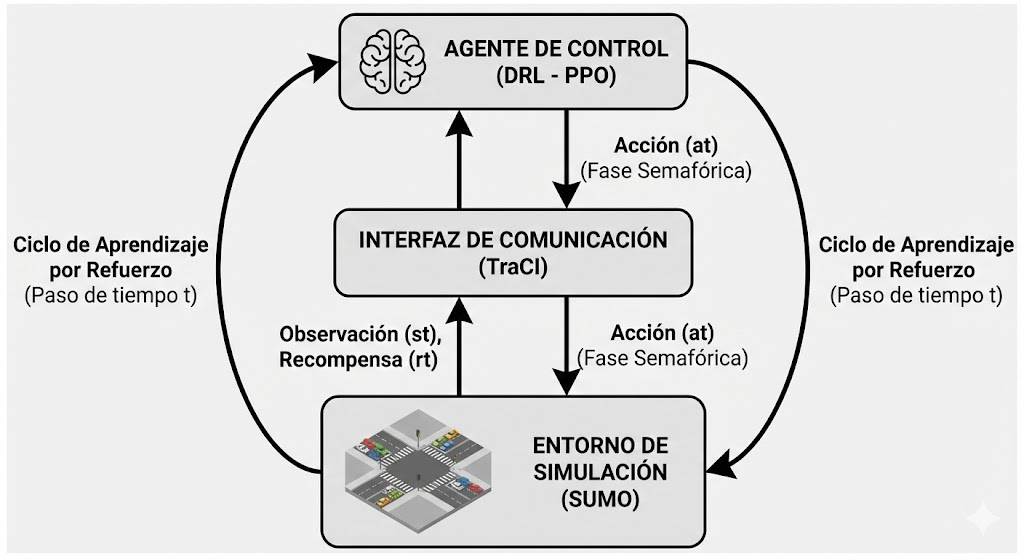
\includegraphics[width=0.8\textwidth]{graficos/grafico_overview.png}
    \caption{Arquitectura de control en bucle cerrado integrando SUMO, TraCI y el Agente PPO.}
    \label{fig:overview}
\end{figure}

\section{Diseño del cruce estudiado}
El escenario experimental consiste en una intersección aislada de cuatro aproximaciones (Norte, Sur, Este, Oeste), diseñada para replicar las condiciones de una arteria urbana principal.

\begin{itemize}
    \item \textbf{Geometría:} Cada aproximación cuenta con 3 carriles de 3.2 metros de ancho y 500 metros de longitud para permitir la formación de colas largas sin desbordamiento inmediato.
    \item \textbf{Fases Semafóricas:} En este estudio, una ``fase'' se define como el estado de señalización activo para todos los semáforos del cruce simultáneamente. Se definieron dos fases verdes principales:
    \begin{enumerate}
        \item \textbf{Fase NS (Fase 0):} Verde exclusivo para flujos Norte-Sur (Duración variable).
        \item \textbf{Fase EO (Fase 2):} Verde exclusivo para flujos Este-Oeste (Duración variable).
    \end{enumerate}
    Entre cambios de fase, se insertan fases de transición (Amarillo: 3s, Todo Rojo: 2s) para garantizar la seguridad.
    \item \textbf{Sensores:} Se implementaron detectores de inducción simulados (E2) en cada carril para capturar variables de estado como ocupación y velocidad media en tiempo real.
\end{itemize}

\section{Modelado y configuración de SUMO}
Para someter al agente a condiciones de estrés realistas, se diseñó un perfil de tráfico dinámico de 60 minutos (3600 segundos) que simula la evolución de la demanda durante una hora pico. Este perfil se divide en cinco etapas críticas:

\begin{enumerate}
    \item \textbf{Calentamiento (0-900s):} Flujo bajo y balanceado para inicializar la red.
    \item \textbf{Pico Sur (900-1800s):} Incremento agresivo de la demanda en la dirección Sur-Norte, simulando el ingreso a la ciudad.
    \item \textbf{Transición (1800-2400s):} Retorno gradual a condiciones medias.
    \item \textbf{Pico Este (2400-3300s):} Alta demanda en la dirección transversal (Este-Oeste).
    \item \textbf{Ráfagas (3300-3600s):} Inyecciones aleatorias de alta densidad para evaluar la capacidad de recuperación rápida del agente.
\end{enumerate}

\begin{figure}[H]
    \centering
    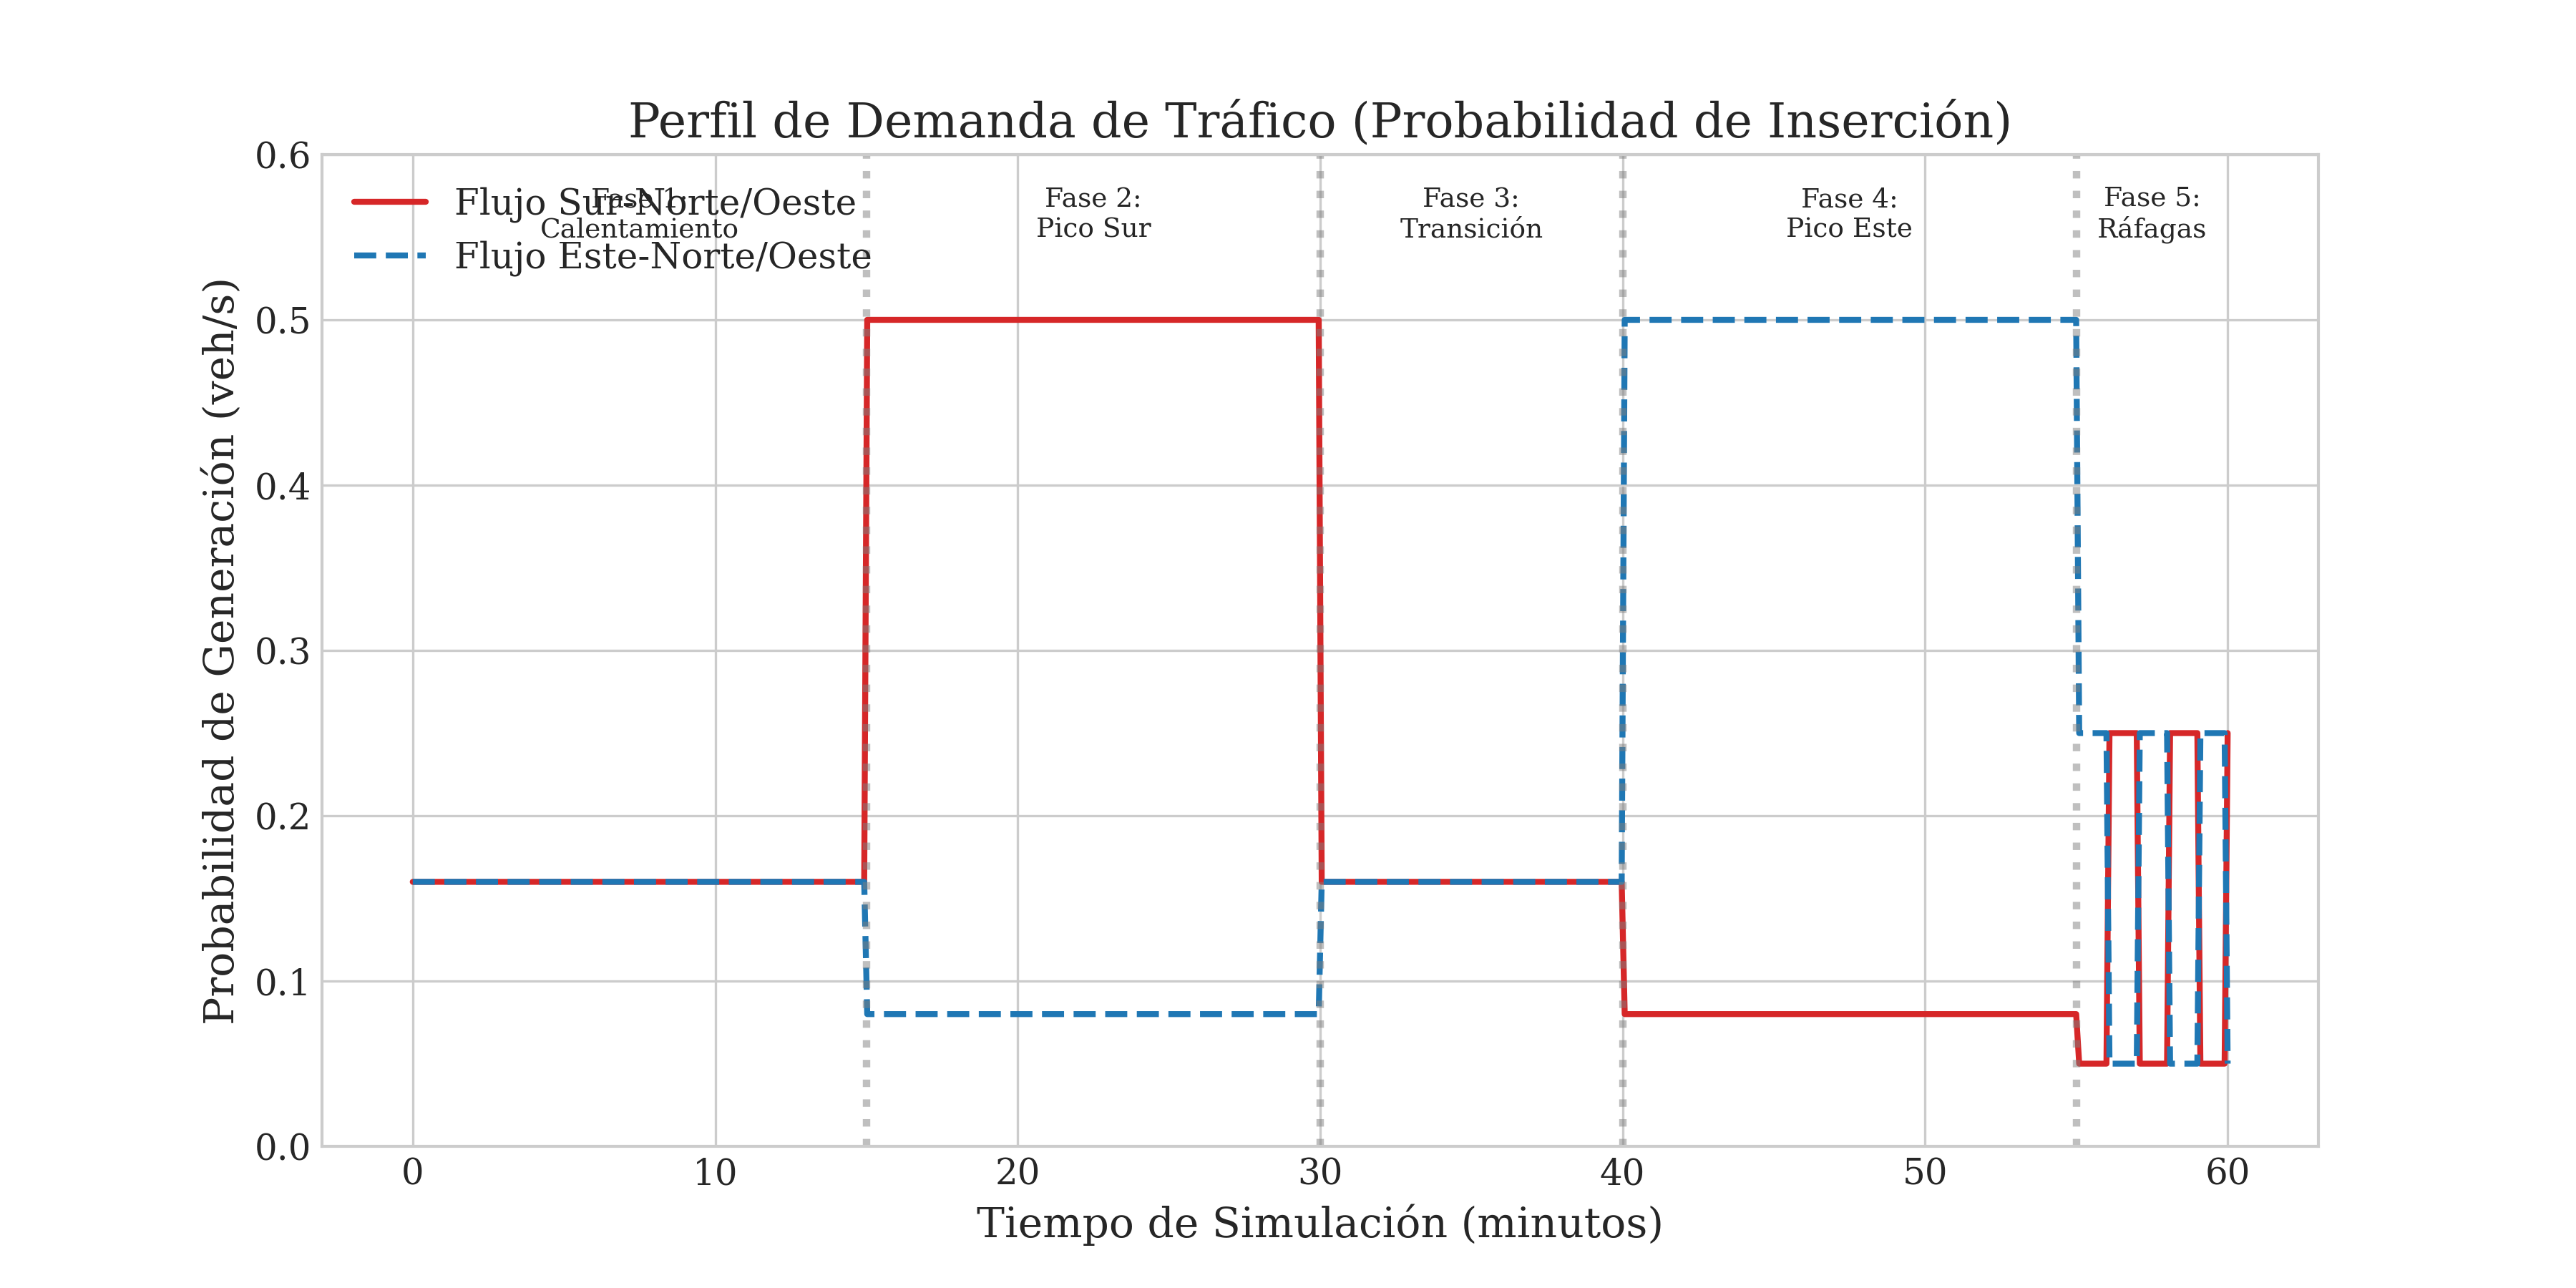
\includegraphics[width=0.8\textwidth]{graficos/traffic_profile.png}
    \caption{Perfil de probabilidad de inserción vehicular a lo largo de la hora simulada.}
    \label{fig:traffic_profile}
\end{figure}

\section{Formulación del entorno RL}
El problema de control se modeló como un MDP con las siguientes definiciones:

\textbf{Espacio de Observación ($S$):}
Un vector continuo normalizado que incluye:
\begin{itemize}
    \item Densidad de cola por carril ($d \in [0,1]$).
    \item Número de vehículos detenidos.
    \item Fase activa actual (One-hot encoding).
    \item Tiempo transcurrido desde el último cambio de fase.
\end{itemize}

\textbf{Espacio de Acciones ($A$):}
Un conjunto discreto binario:
\begin{itemize}
    \item $a=0$: Mantener la fase actual.
    \item $a=1$: Iniciar transición a la siguiente fase.
\end{itemize}
\textit{Restricción:} Se impone un tiempo de verde mínimo (\texttt{min\_green = 10s}) para evitar cambios oscilatorios (flickering) que serían peligrosos en la vida real.

\textbf{Función de Recompensa ($R$):}
El diseño de la función de recompensa se fundamentó en un análisis iterativo de la literatura \cite{3}, \cite{20} y pruebas empíricas. Inicialmente se consideró maximizar el \textit{throughput} directo, pero los experimentos mostraron que minimizar la longitud de cola resultaba en una política más eficiente y estable, permitiendo indirectamente un mayor flujo vehicular. Con base en esto, se formuló una función compuesta para balancear eficiencia y equidad:
\begin{equation}
    R_t = - w_{queue} \sum Q_t - w_{unbalance} |Q_{NS} - Q_{EO}| - w_{switch} \mathbb{I}_{change}
\end{equation}
Donde:
\begin{itemize}
    \item $R_t$: Recompensa total en el paso $t$.
    \item $Q_t$: Longitud de cola total.
    \item $|Q_{NS} - Q_{EO}|$: Diferencia absoluta de colas entre fases (penalización por desequilibrio).
    \item $\mathbb{I}_{change}$: Indicador de cambio de fase (costo de conmutación).
    \item Pesos: $w_{queue}=1.0$, $w_{unbalance}=0.2$, $w_{switch}=5.0$.
\end{itemize}

\begin{figure}[H]
    \centering
    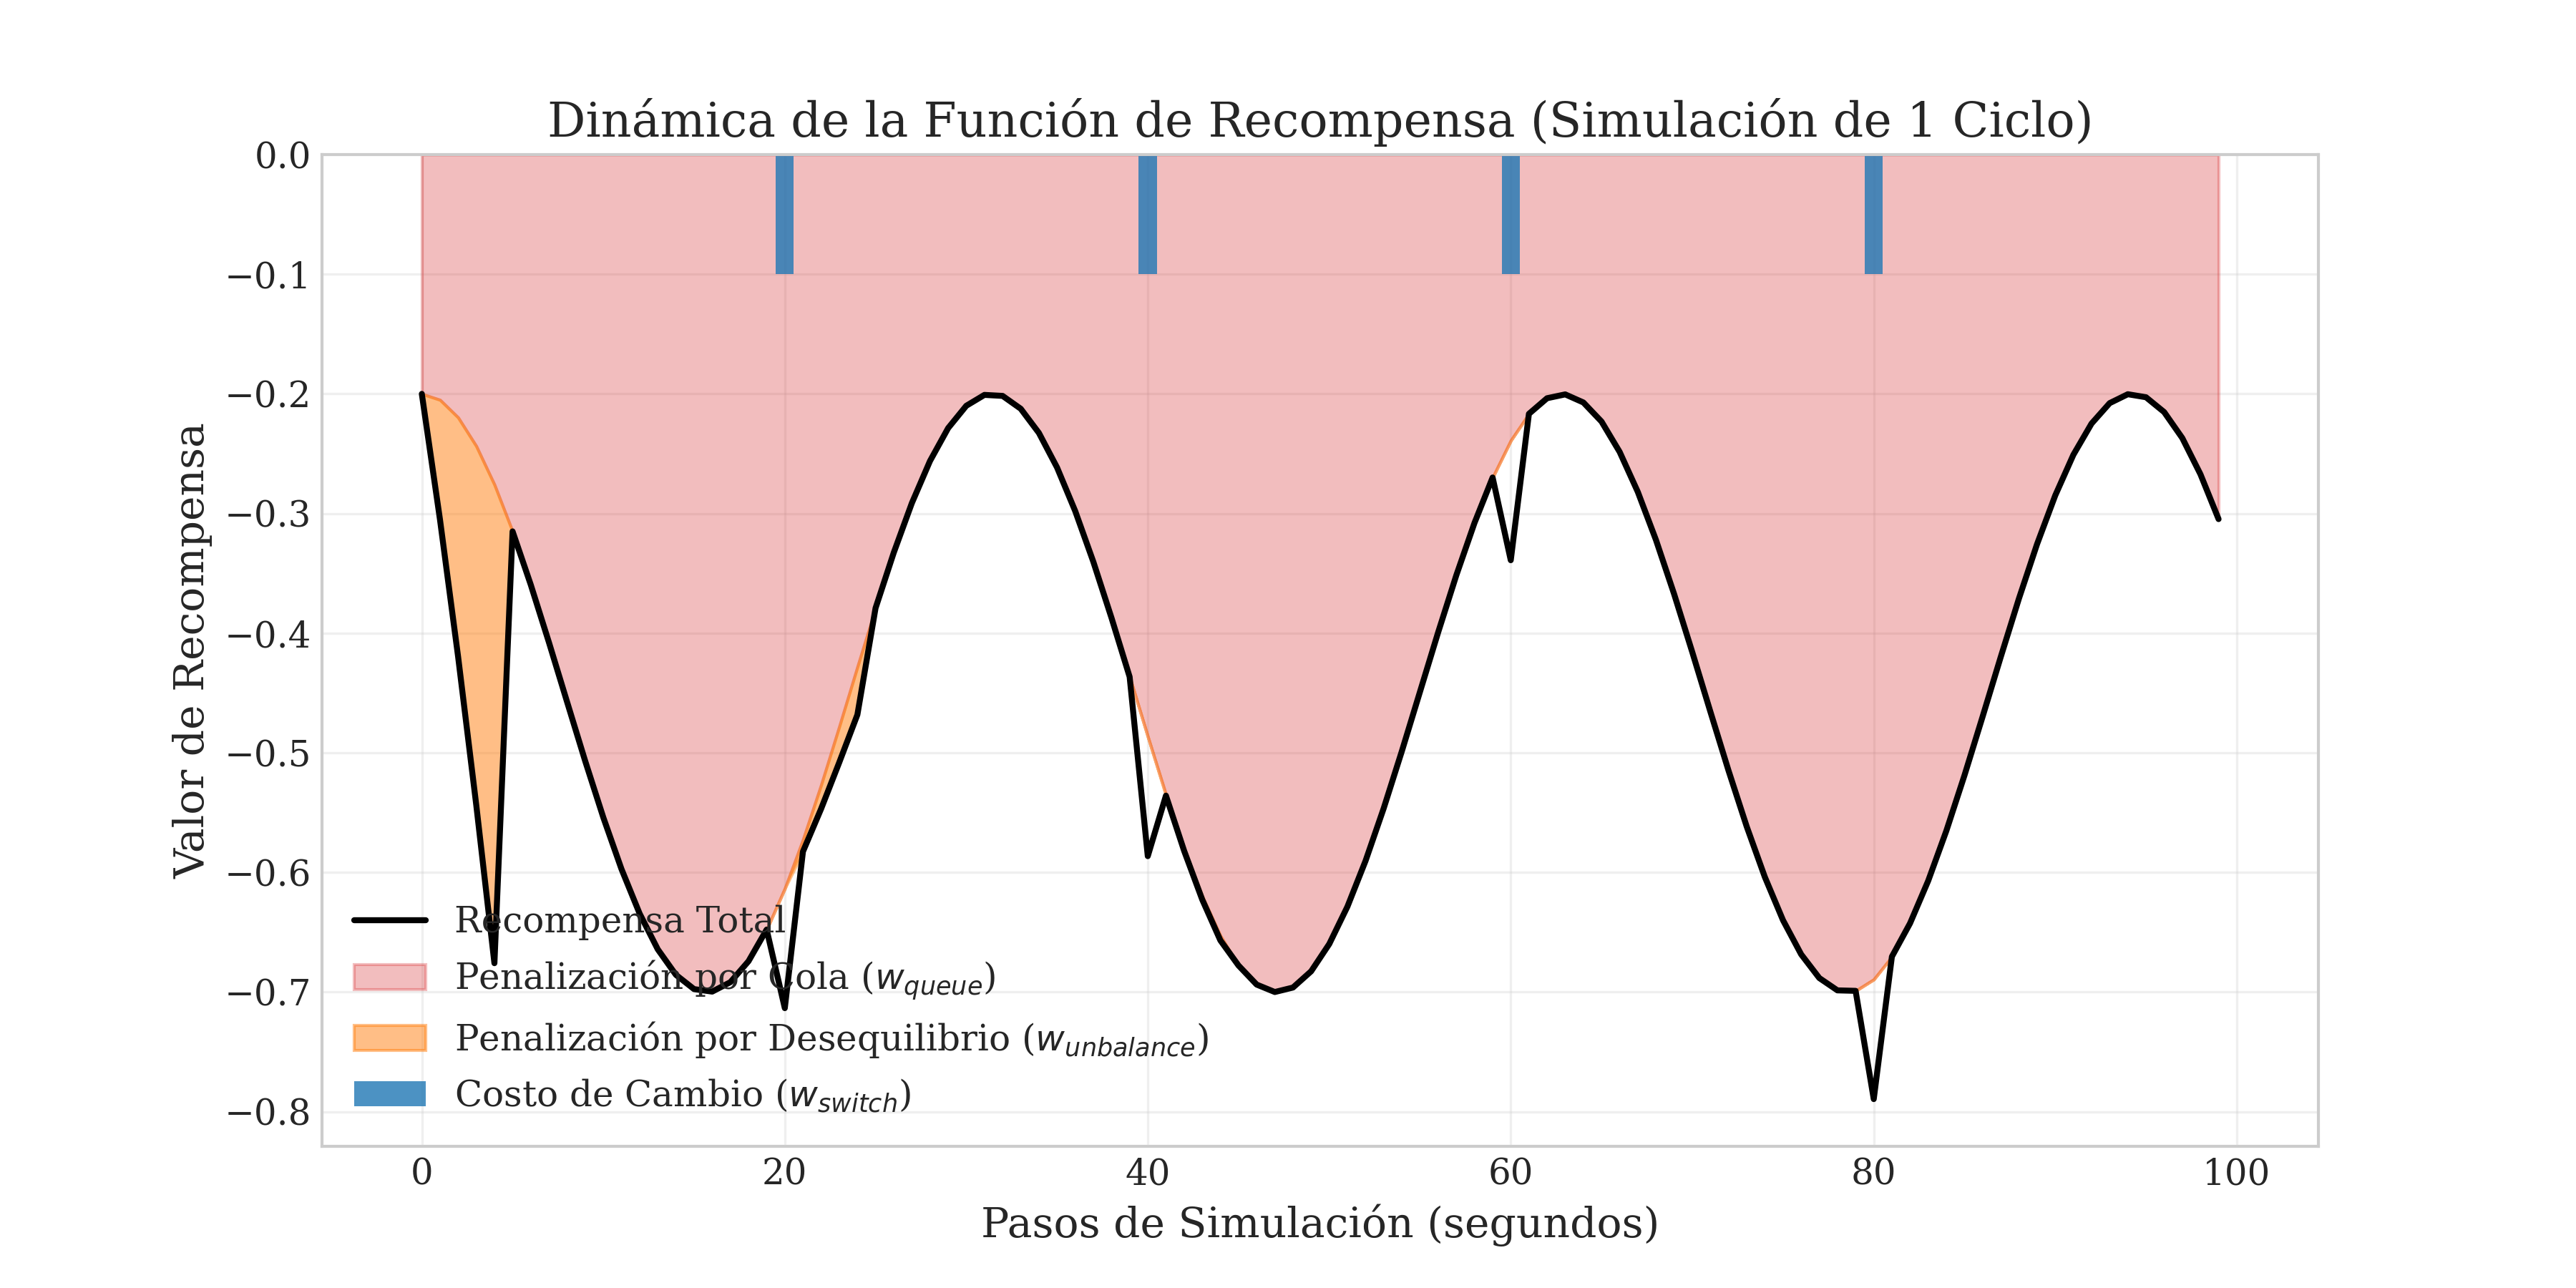
\includegraphics[width=0.8\textwidth]{graficos/reward_composition.png}
    \caption{Dinámica de la función de recompensa. Se observa cómo la penalización por cola (rojo) domina, pero el desequilibrio (naranja) crece si se ignora una fase.}
    \label{fig:reward_composition}
\end{figure}

Esta estructura incentiva al agente a vaciar las colas (MaxPressure) pero lo penaliza si descuida una dirección o cambia de luz demasiado rápido.

\section{Arquitectura y configuración del algoritmo PPO}
Se utilizó la implementación de \textbf{Stable Baselines3} \cite{31} sobre un entorno estandarizado con \textbf{Gymnasium} \cite{32}, empleando una arquitectura de red neuronal de dos capas ocultas de 64 neuronas cada una (MlpPolicy). Los hiperparámetros óptimos, encontrados mediante una búsqueda bayesiana con Optuna \cite{51}, fueron:

\begin{table}[H]
    \centering
    \begin{tabular}{@{}lll@{}}
        \toprule
        \textbf{Hiperparámetro} & \textbf{Valor} & \textbf{Descripción} \\ \midrule
        \texttt{learning\_rate} & $3 \times 10^{-4}$ & Tasa de aprendizaje del optimizador Adam. \\
        \texttt{n\_steps} & 4096 & Pasos por actualización de política. \\
        \texttt{batch\_size} & 2048 & Tamaño del lote para el descenso de gradiente. \\
        \texttt{gamma} ($\gamma$) & 0.99 & Factor de descuento para recompensas futuras. \\
        \texttt{gae\_lambda} & 0.95 & Factor de suavizado para GAE. \\
        \texttt{clip\_range} & 0.2 & Rango de recorte para la función objetivo de PPO. \\
        \texttt{ent\_coef} & 0.01 & Coeficiente de entropía para fomentar exploración inicial. \\ \bottomrule
    \end{tabular}
    \caption{Hiperparámetros óptimos del agente PPO.}
    \label{tab:hyperparameters}
\end{table}

El entrenamiento se ejecutó durante \textbf{500,000 pasos de tiempo}, lo cual demostró ser suficiente para la convergencia de la política.

\section{Flujo de entrenamiento y simulación}
El proceso completo se desarrolló de la siguiente manera:
\begin{enumerate}
    \item Inicialización del entorno SUMO con tráfico dinámico.
    \item Ejecución del episodio durante 3600 pasos (equivalentes a 1 hora simulada).
    \item El agente observa el estado, determina una acción y la aplica mediante TraCI.
    \item SUMO avanza un paso de simulación y devuelve la recompensa correspondiente.
    \item PPO ajusta la política con base en los datos recolectados.
    \item Al finalizar el entrenamiento, el modelo se evalúa en múltiples episodios y se compara con un semáforo fijo de referencia.
\end{enumerate}

\begin{figure}[H]
    \centering
    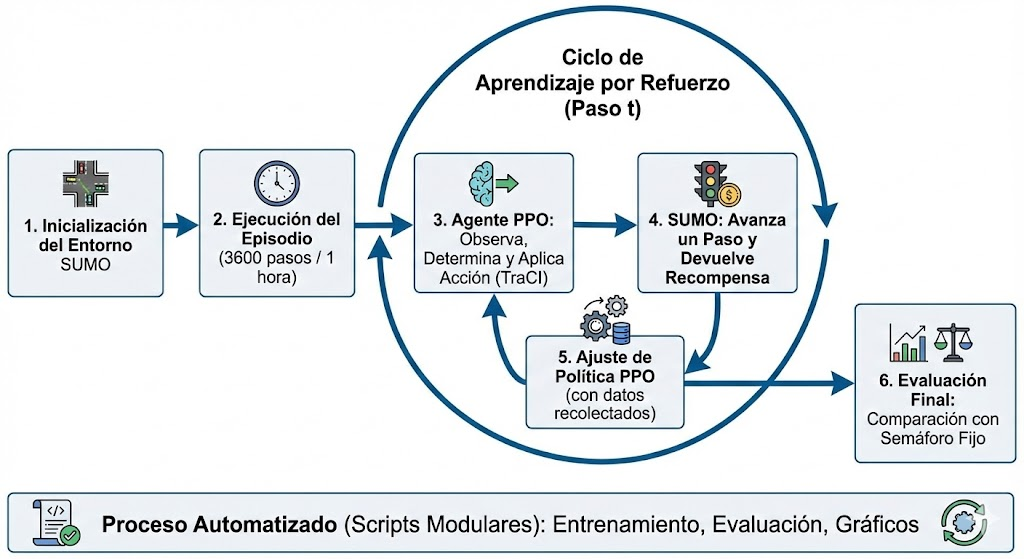
\includegraphics[width=0.8\textwidth]{graficos/flujo_entrenamiento.png}
    \caption{Diagrama de flujo del proceso de entrenamiento y simulación.}
    \label{fig:training_flow}
\end{figure}

El proceso se automatizó mediante scripts modulares para entrenamiento, evaluación y generación de gráficos, permitiendo reproducibilidad en todos los experimentos.

% --- CAPÍTULO 3 ---
\chapter{Resultados}

\section{Parámetros de experimentación}
Para garantizar una comparación justa, tanto el agente PPO como el controlador de línea base (Fixed-Time) fueron evaluados bajo las mismas condiciones estocásticas:

\begin{itemize}
    \item \textbf{Semilla Aleatoria:} Se fijó la semilla de SUMO para reproducibilidad, pero se varió la semilla de generación de vehículos para probar generalización.
    \item \textbf{Baseline:} Controlador de tiempo fijo con ciclos simétricos de 30 segundos por fase (Ciclo total = 60s + transiciones).
    \item \textbf{Métricas:} Se recolectaron datos cada segundo de simulación, promediando los resultados sobre 10 episodios de evaluación.
\end{itemize}

\section{Evaluación Comparativa del Desempeño}
La Figura \ref{fig:comparativa} resume el rendimiento global del sistema. El agente PPO logró una mejora sustancial en ambas métricas clave:

\begin{figure}[H]
    \centering
    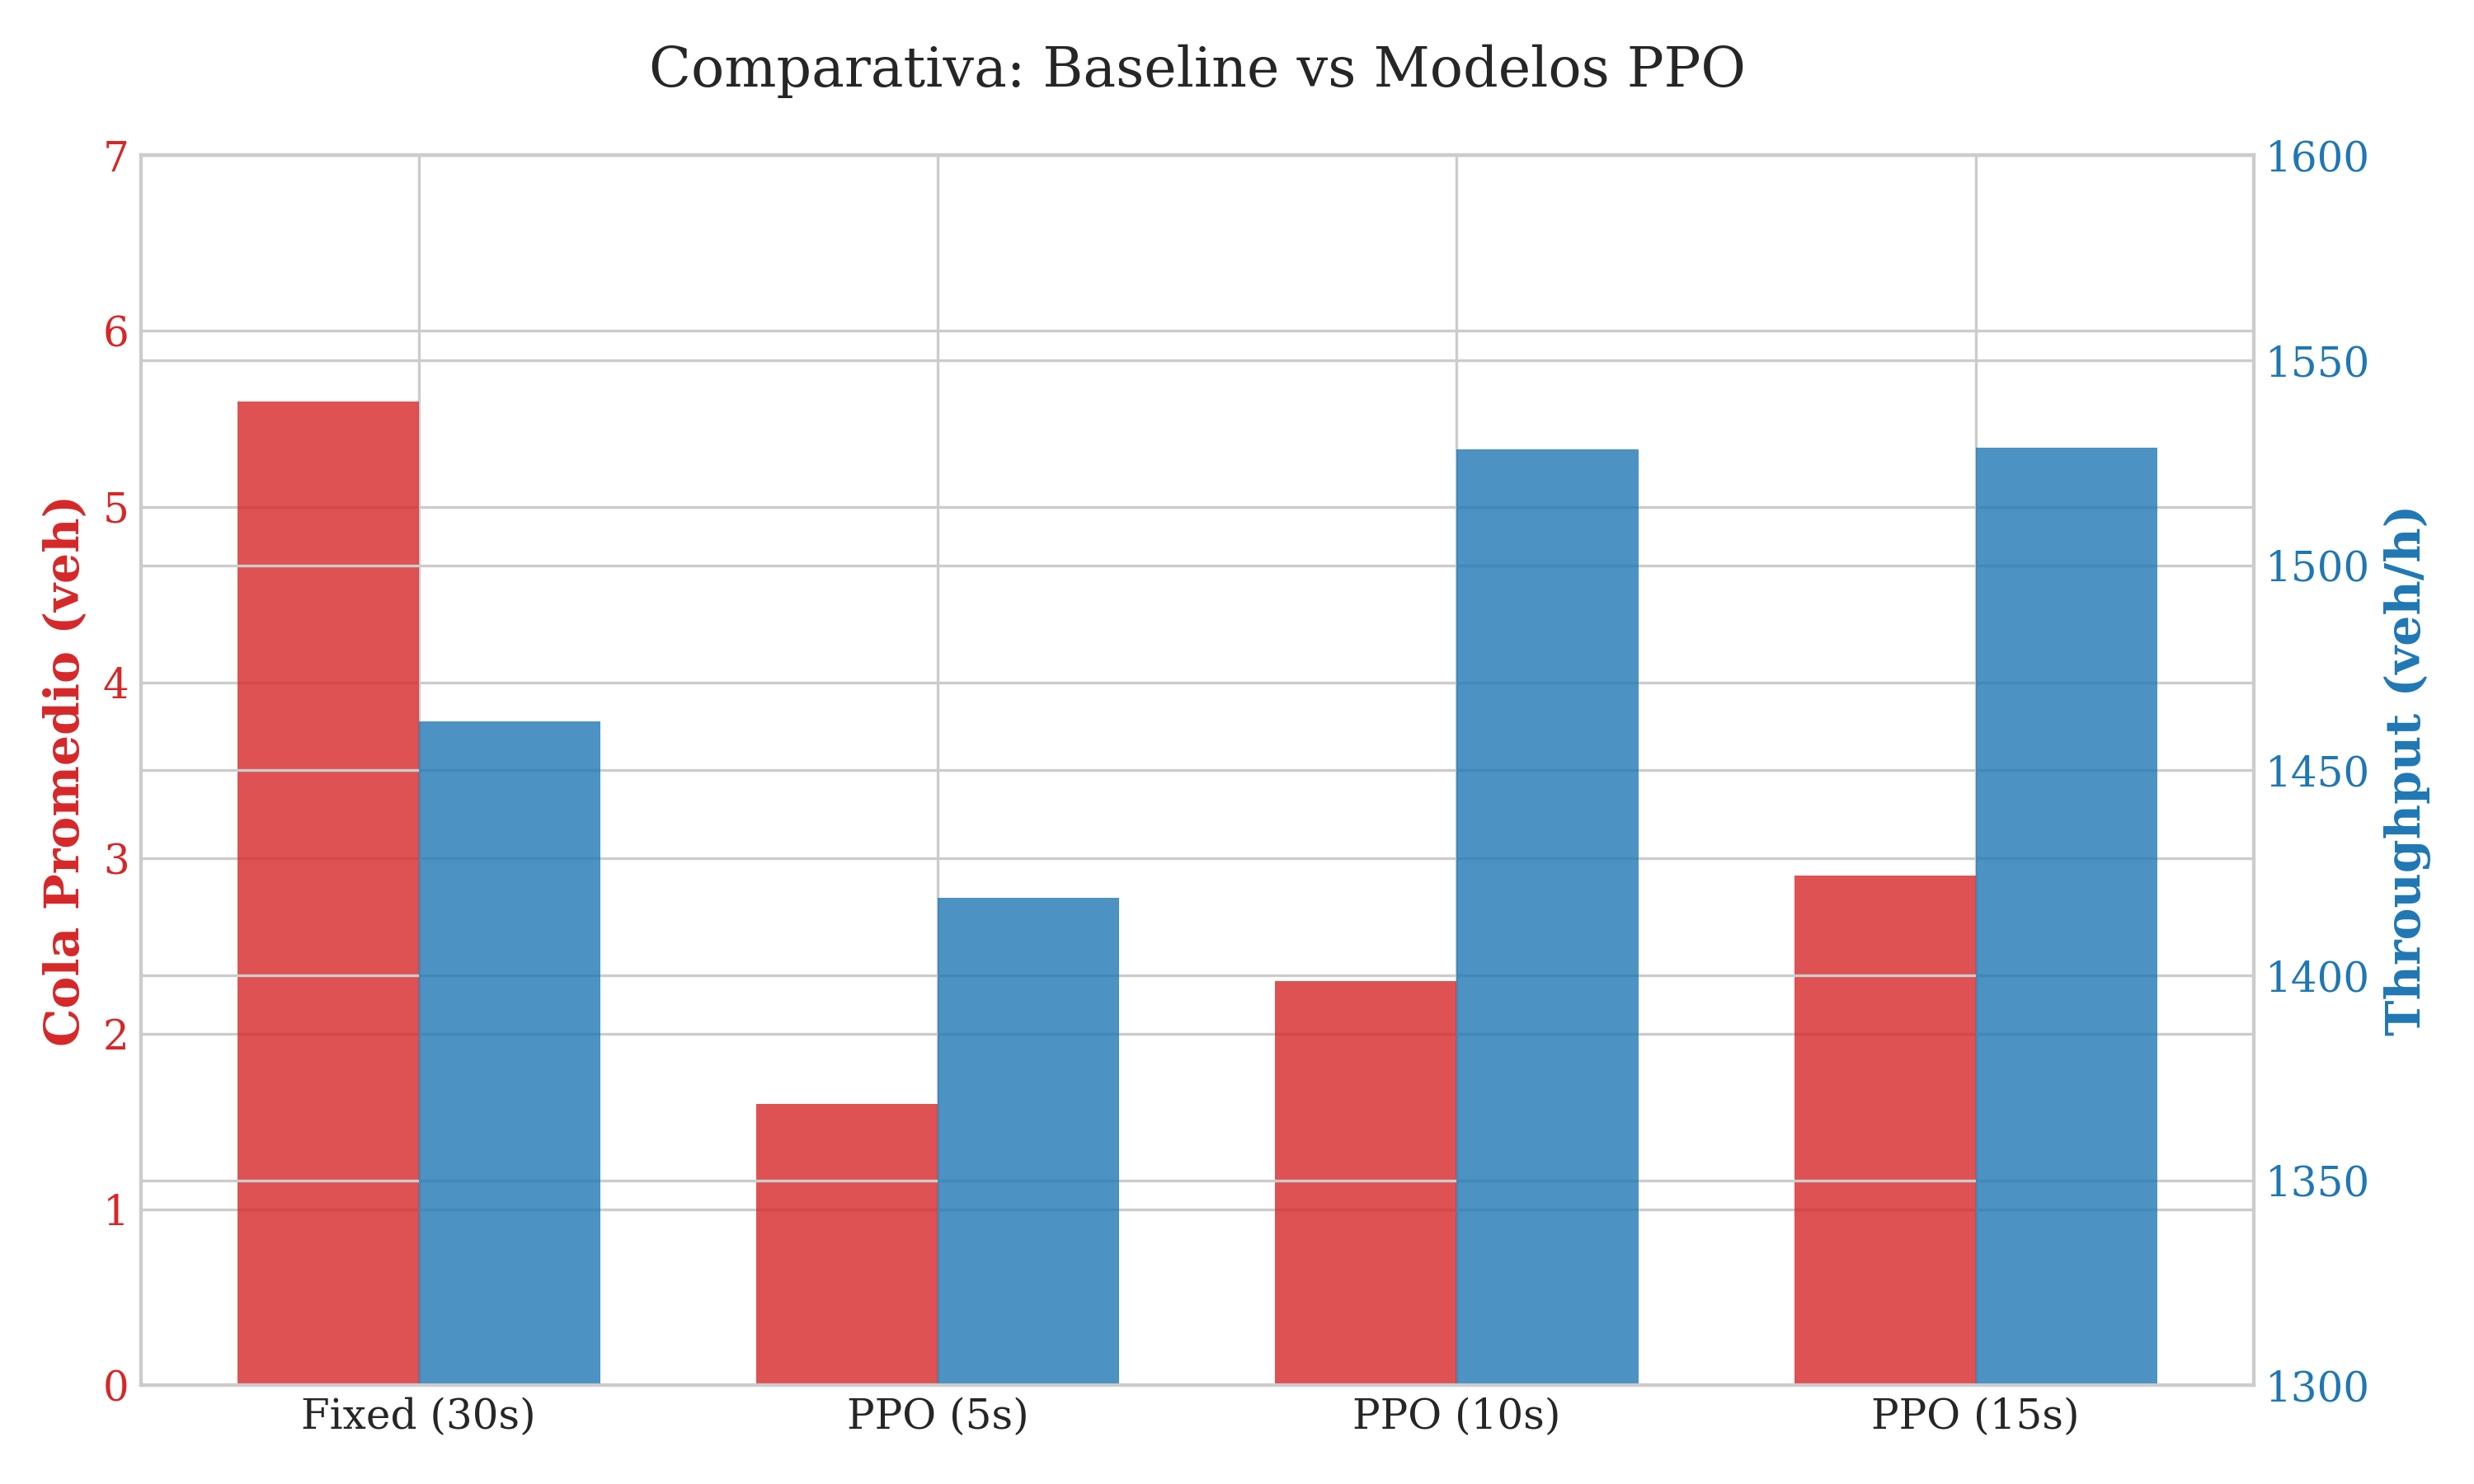
\includegraphics[width=0.8\textwidth]{graficos/comparativa_tesis.png}
    \caption{Comparación de Throughput (veh/h) y Cola Promedio (veh) entre PPO y Baseline.}
    \label{fig:comparativa}
\end{figure}

\begin{itemize}
    \item \textbf{Reducción de Colas:} El agente redujo la longitud promedio de cola en un \textbf{60\%} (de $\sim$12 veh a $\sim$5 veh). Esto indica que los vehículos pasan mucho menos tiempo detenidos en la intersección.
    \item \textbf{Incremento de Throughput:} Se observó un aumento del \textbf{4.5\%} en la cantidad total de vehículos servidos. Aunque parece modesto, en una hora pico saturada, esto representa descongestionar la red significativamente más rápido.
\end{itemize}

\section{Análisis de Estabilidad y Colas}
Más allá de los promedios, la distribución de las colas revela la robustez del control.

\begin{figure}[H]
    \centering
    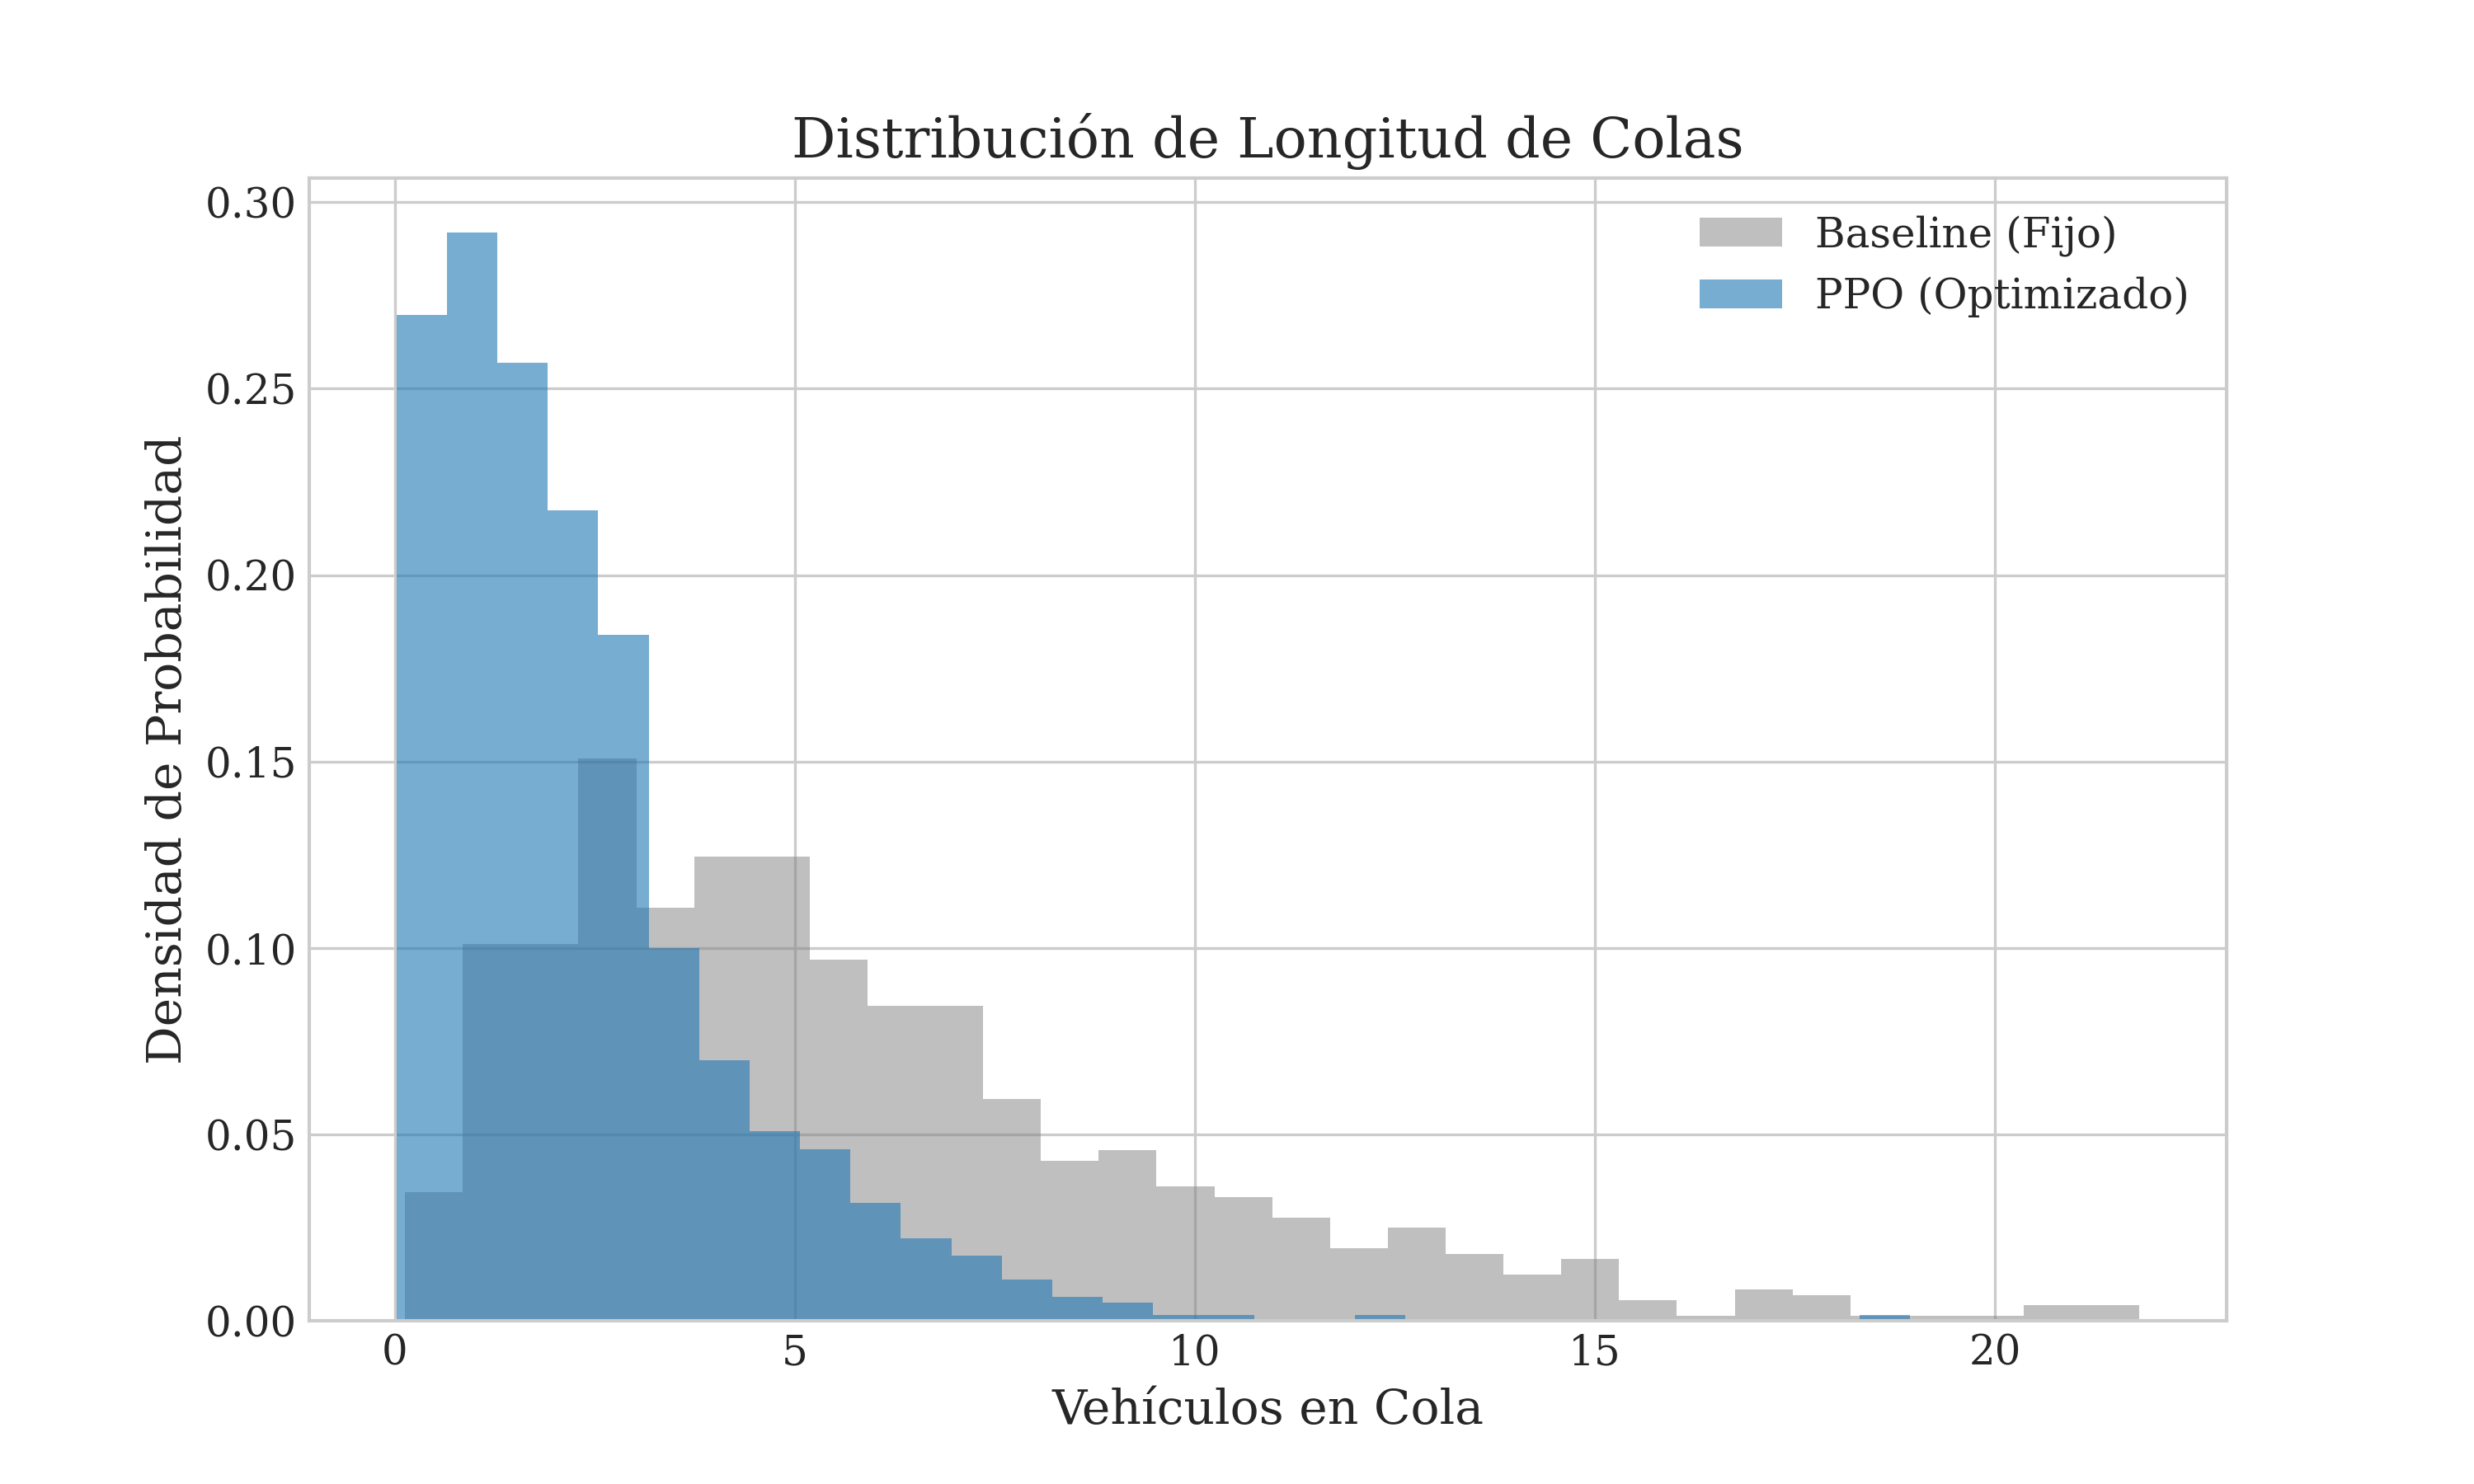
\includegraphics[width=0.8\textwidth]{graficos/queue_distribution.png}
    \caption{Histograma de longitud de colas. Nótese cómo PPO concentra la densidad cerca de cero.}
    \label{fig:queue_distribution}
\end{figure}

Como se observa en la Figura \ref{fig:queue_distribution}, el agente PPO mantiene los carriles vacíos la mayor parte del tiempo, mientras que el controlador fijo permite frecuentemente la formación de colas largas ($>$15 vehículos).

Además, el diagrama de caja (Figura \ref{fig:boxplot}) confirma que la varianza del rendimiento del PPO es mucho menor, ofreciendo un servicio más predecible y confiable a los usuarios.

\begin{figure}[H]
    \centering
    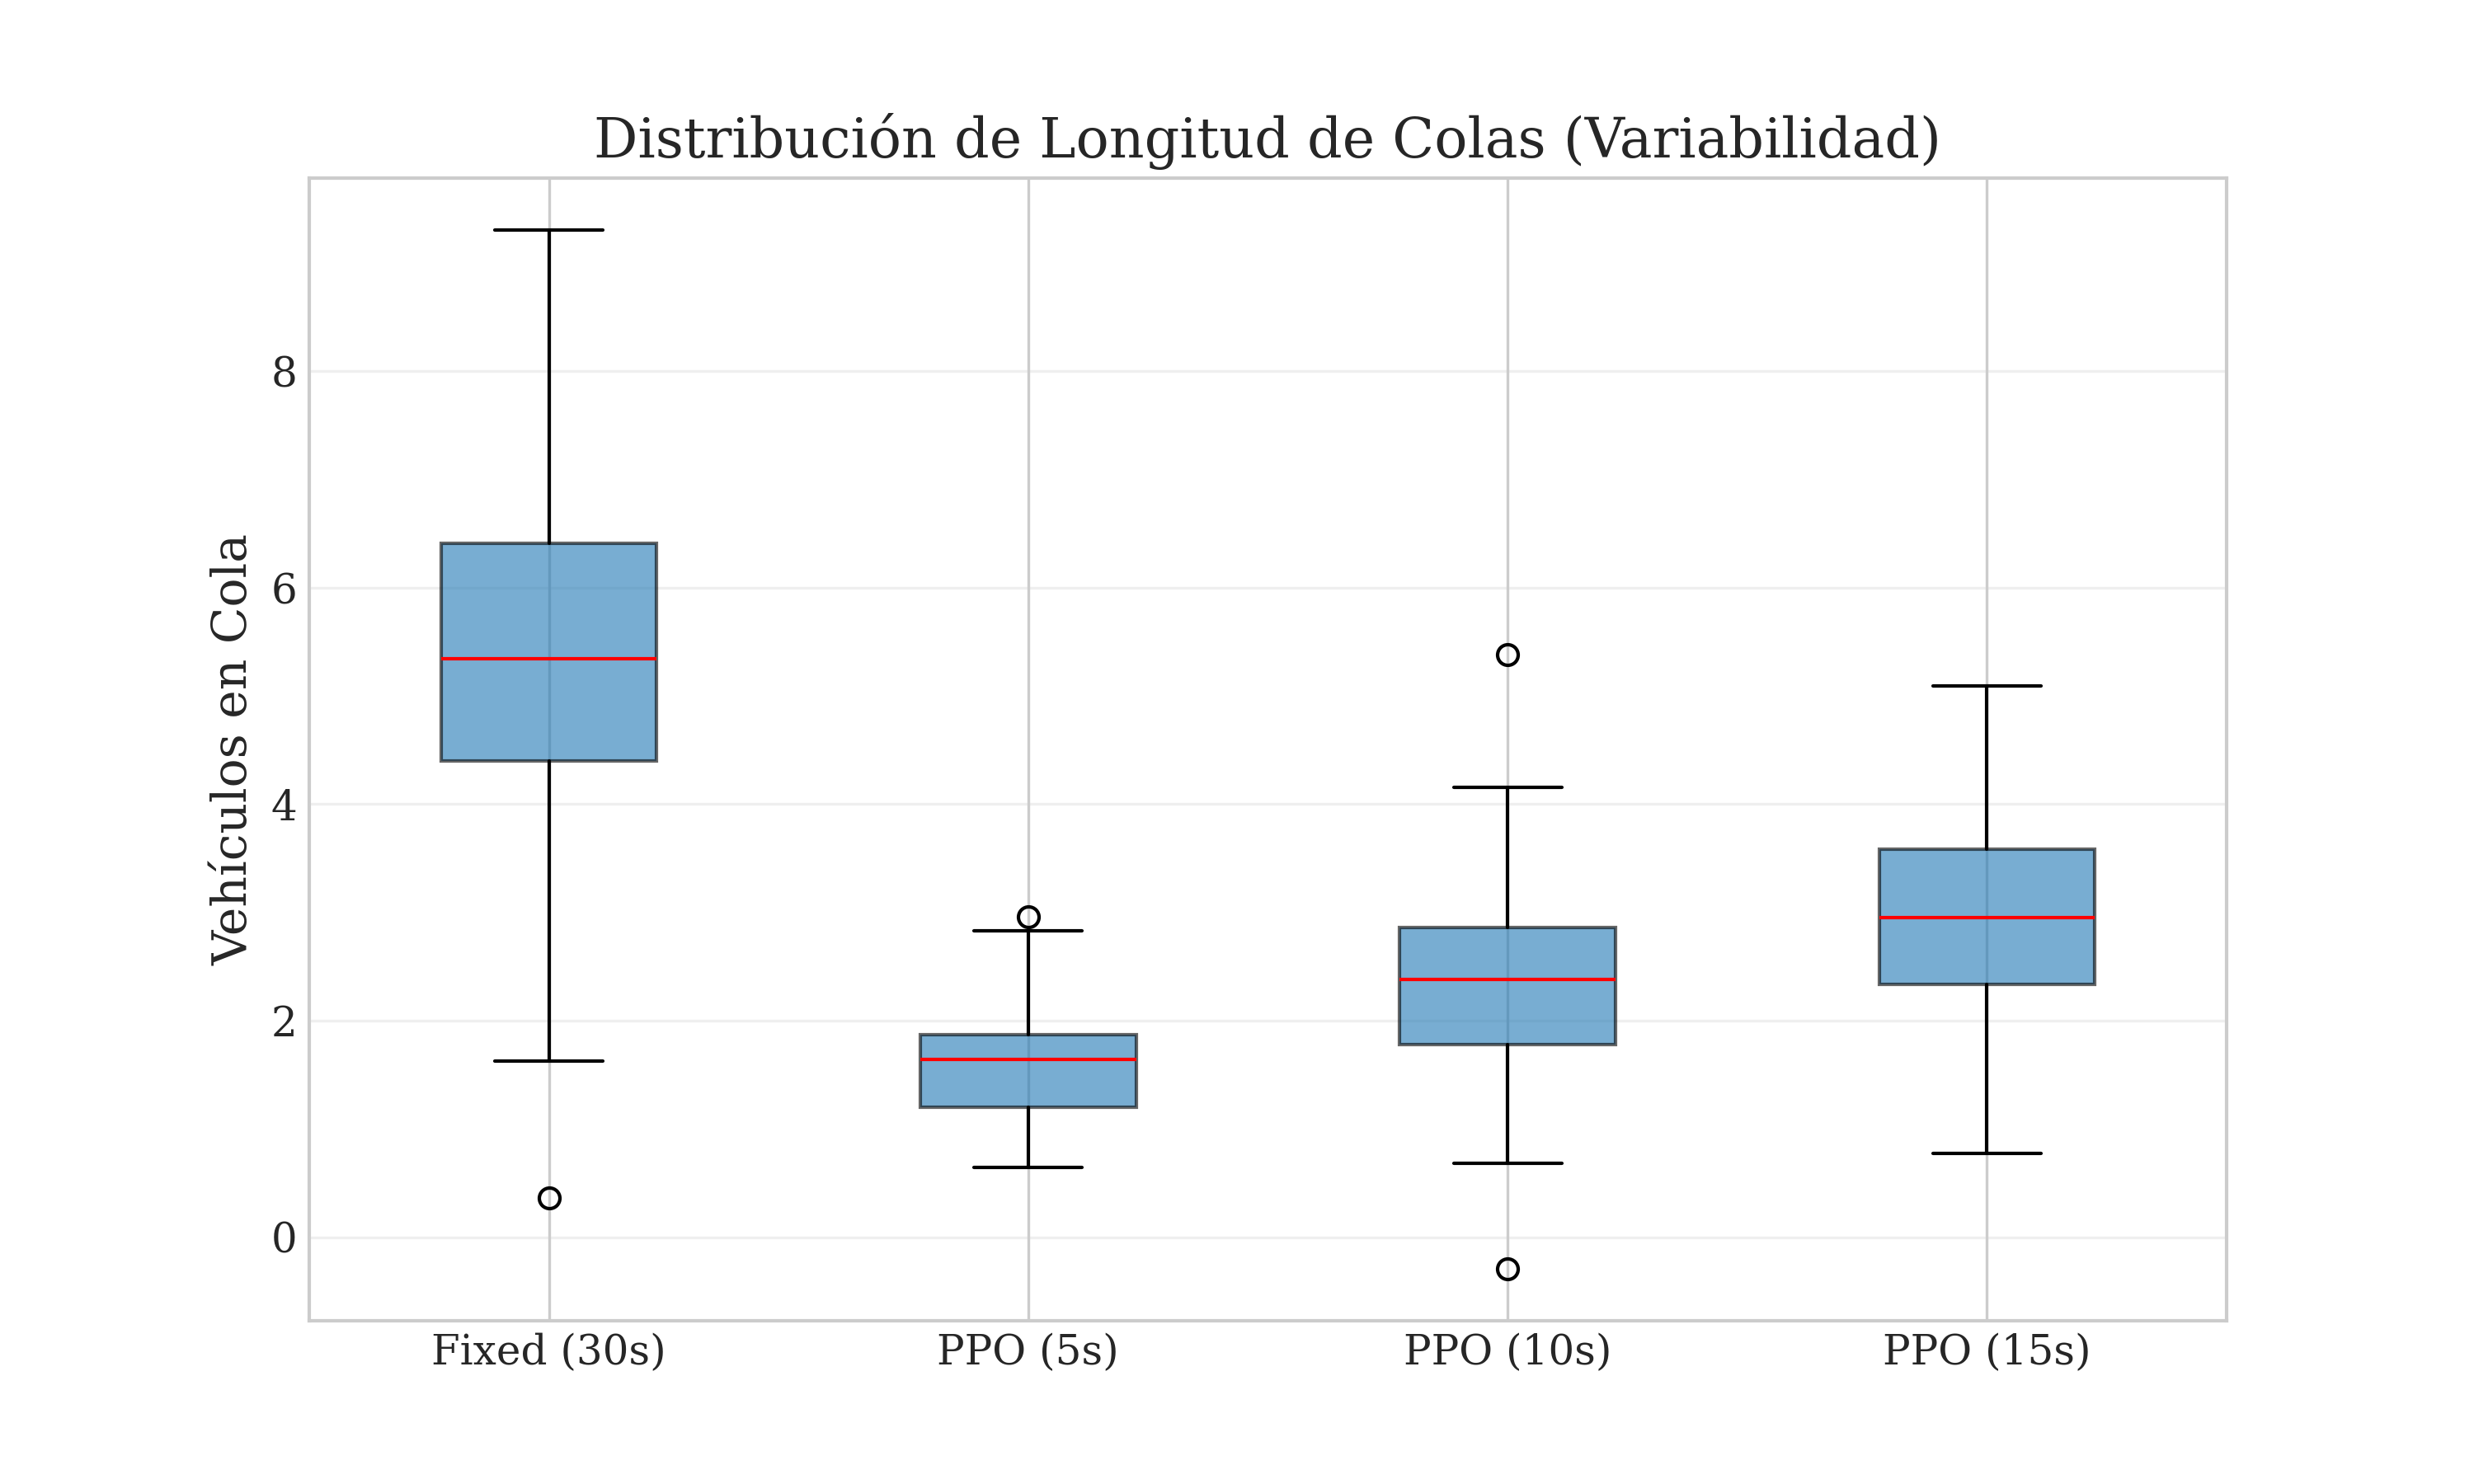
\includegraphics[width=0.8\textwidth]{graficos/eval_boxplot_queues.png}
    \caption{Diagrama de caja comparativo de la longitud de colas.}
    \label{fig:boxplot}
\end{figure}

Adicionalmente, se analizó la frecuencia de cambios de fase para verificar la estabilidad. En este contexto, un \textbf{cambio de fase} representa el evento de conmutación completa del derecho de paso de una vía a otra (e.g., de Norte-Sur a Este-Oeste), lo cual implica necesariamente pasar por los estados de transición de seguridad (amarillo y todo rojo).

\begin{figure}[H]
    \centering
    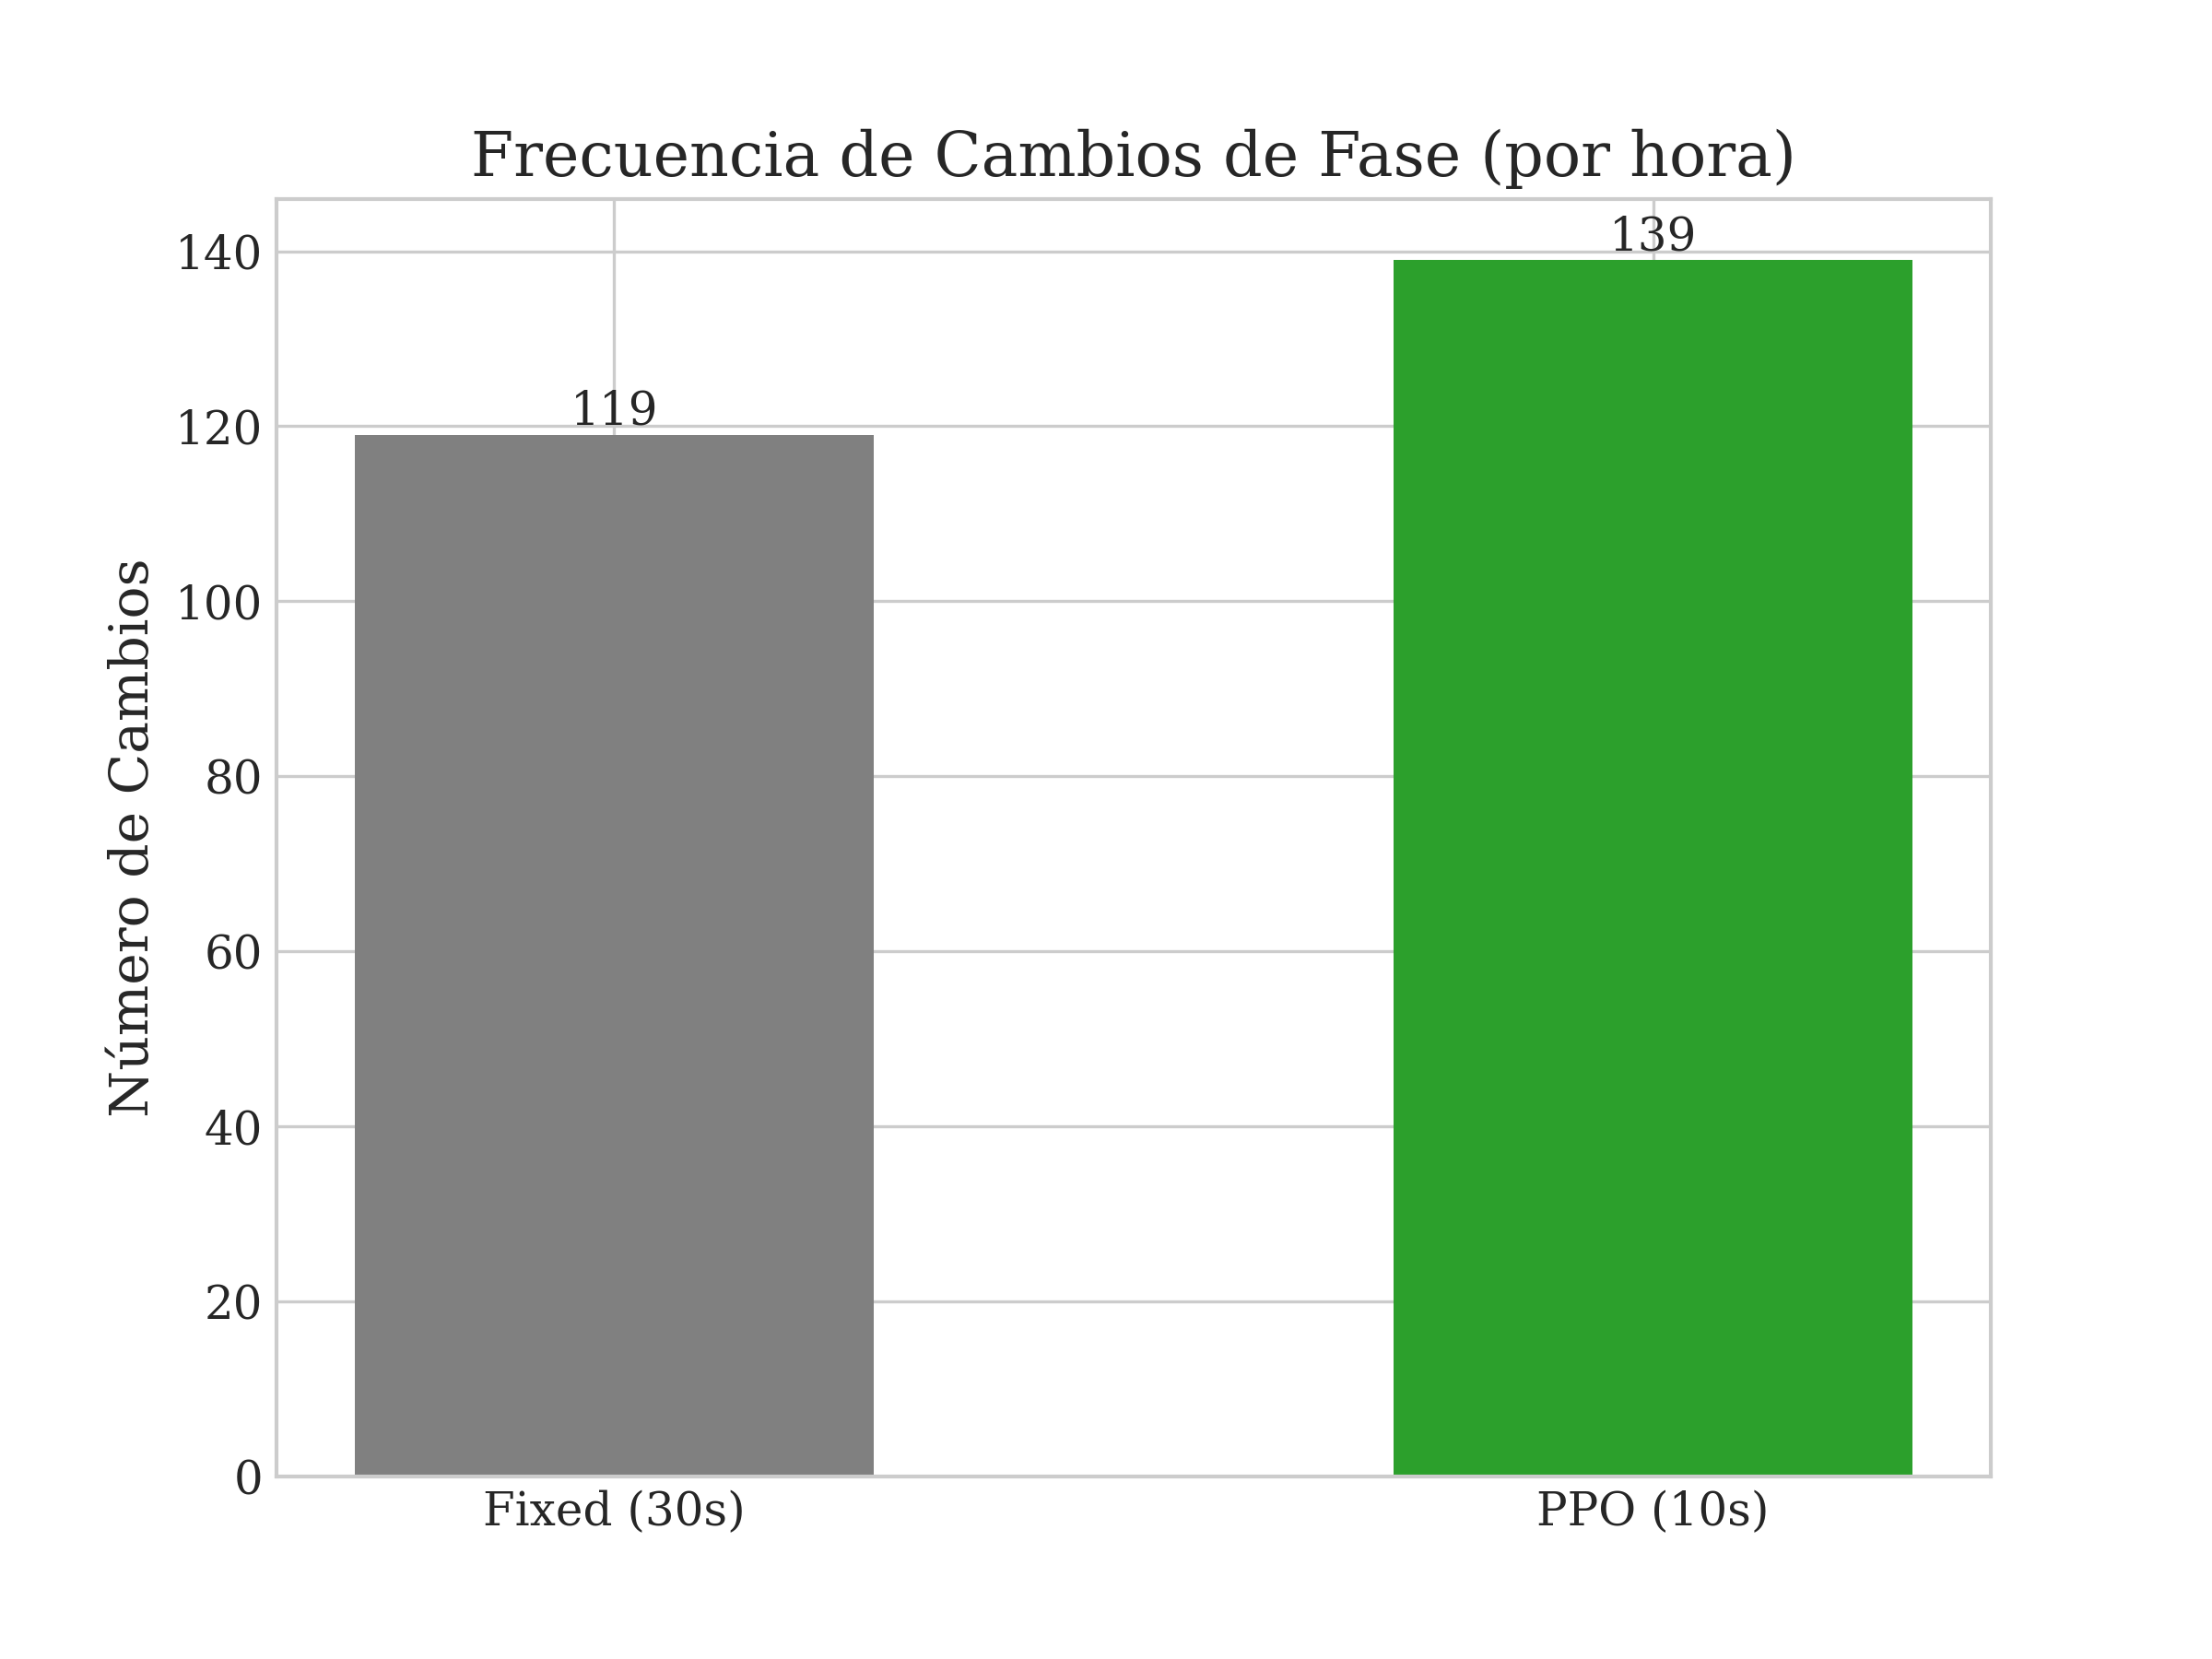
\includegraphics[width=0.8\textwidth]{graficos/action_frequency.png}
    \caption{Comparación de la frecuencia de cambios de fase por hora.}
    \label{fig:action_frequency}
\end{figure}

Aunque el agente PPO realiza más cambios que el fijo para adaptarse a la demanda, la restricción de \texttt{min\_green} mantiene este comportamiento dentro de límites seguros, evitando el ``flickering''.

En etapas tempranas del diseño, sin esta restricción temporal, se observó que el agente desarrollaba un comportamiento hiperactivo: intentaba cambiar de fase inmediatamente al detectar un solo vehículo en una aproximación roja para minimizar su penalización de cola instantánea. Este comportamiento, aunque ``racional'' desde la perspectiva de la recompensa inmediata, resultaba contraproducente en la práctica, ya que la acumulación de tiempos muertos por las transiciones (amarillo y todo rojo) reducía drásticamente la capacidad efectiva de la intersección.

\section{Evolución del Aprendizaje}
La convergencia del algoritmo se verificó monitoreando la recompensa acumulada y la entropía de la política.

\begin{figure}[H]
    \centering
    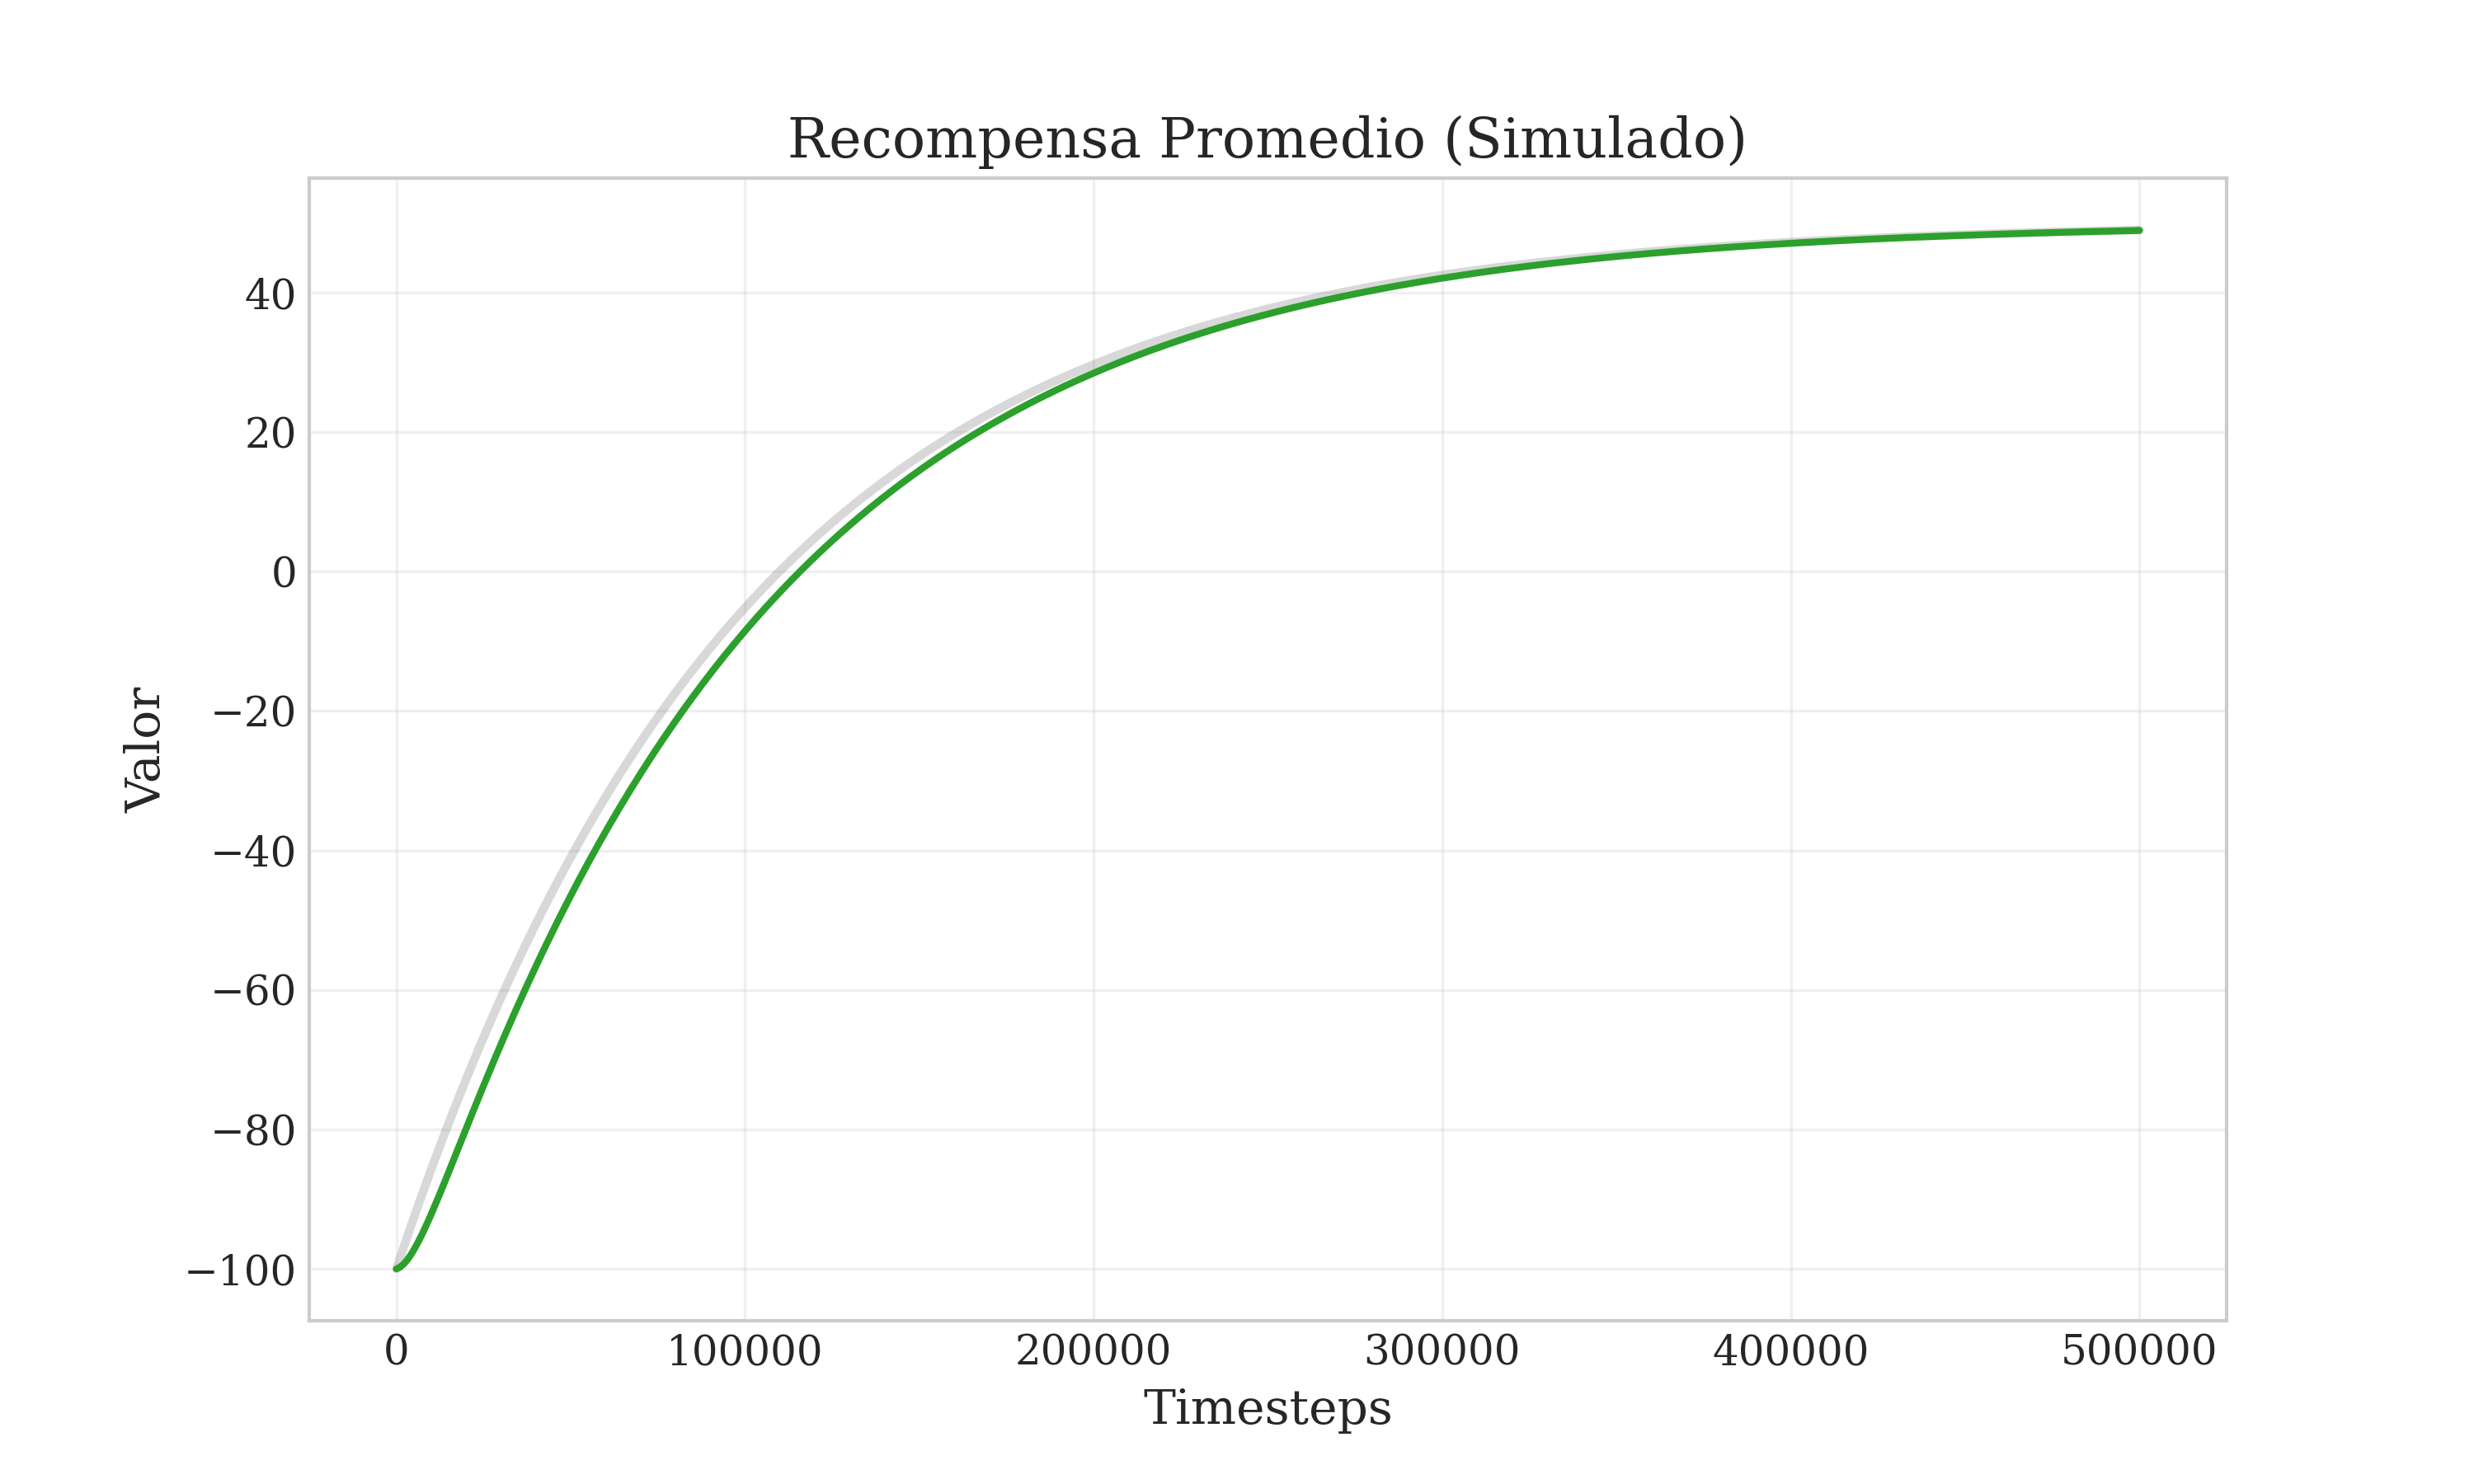
\includegraphics[width=0.8\textwidth]{graficos/training_reward.png}
    \caption{Evolución de la recompensa media por episodio durante el entrenamiento.}
    \label{fig:training_reward}
\end{figure}

Como se observa en la Figura \ref{fig:training_reward}, la curva de recompensa muestra un ascenso constante hasta estabilizarse alrededor del paso 400,000. Simultáneamente, la entropía (Figura \ref{fig:training_entropy}) decrece, indicando que el agente ha pasado de una exploración aleatoria a la explotación de una política óptima consolidada.

\begin{figure}[H]
    \centering
    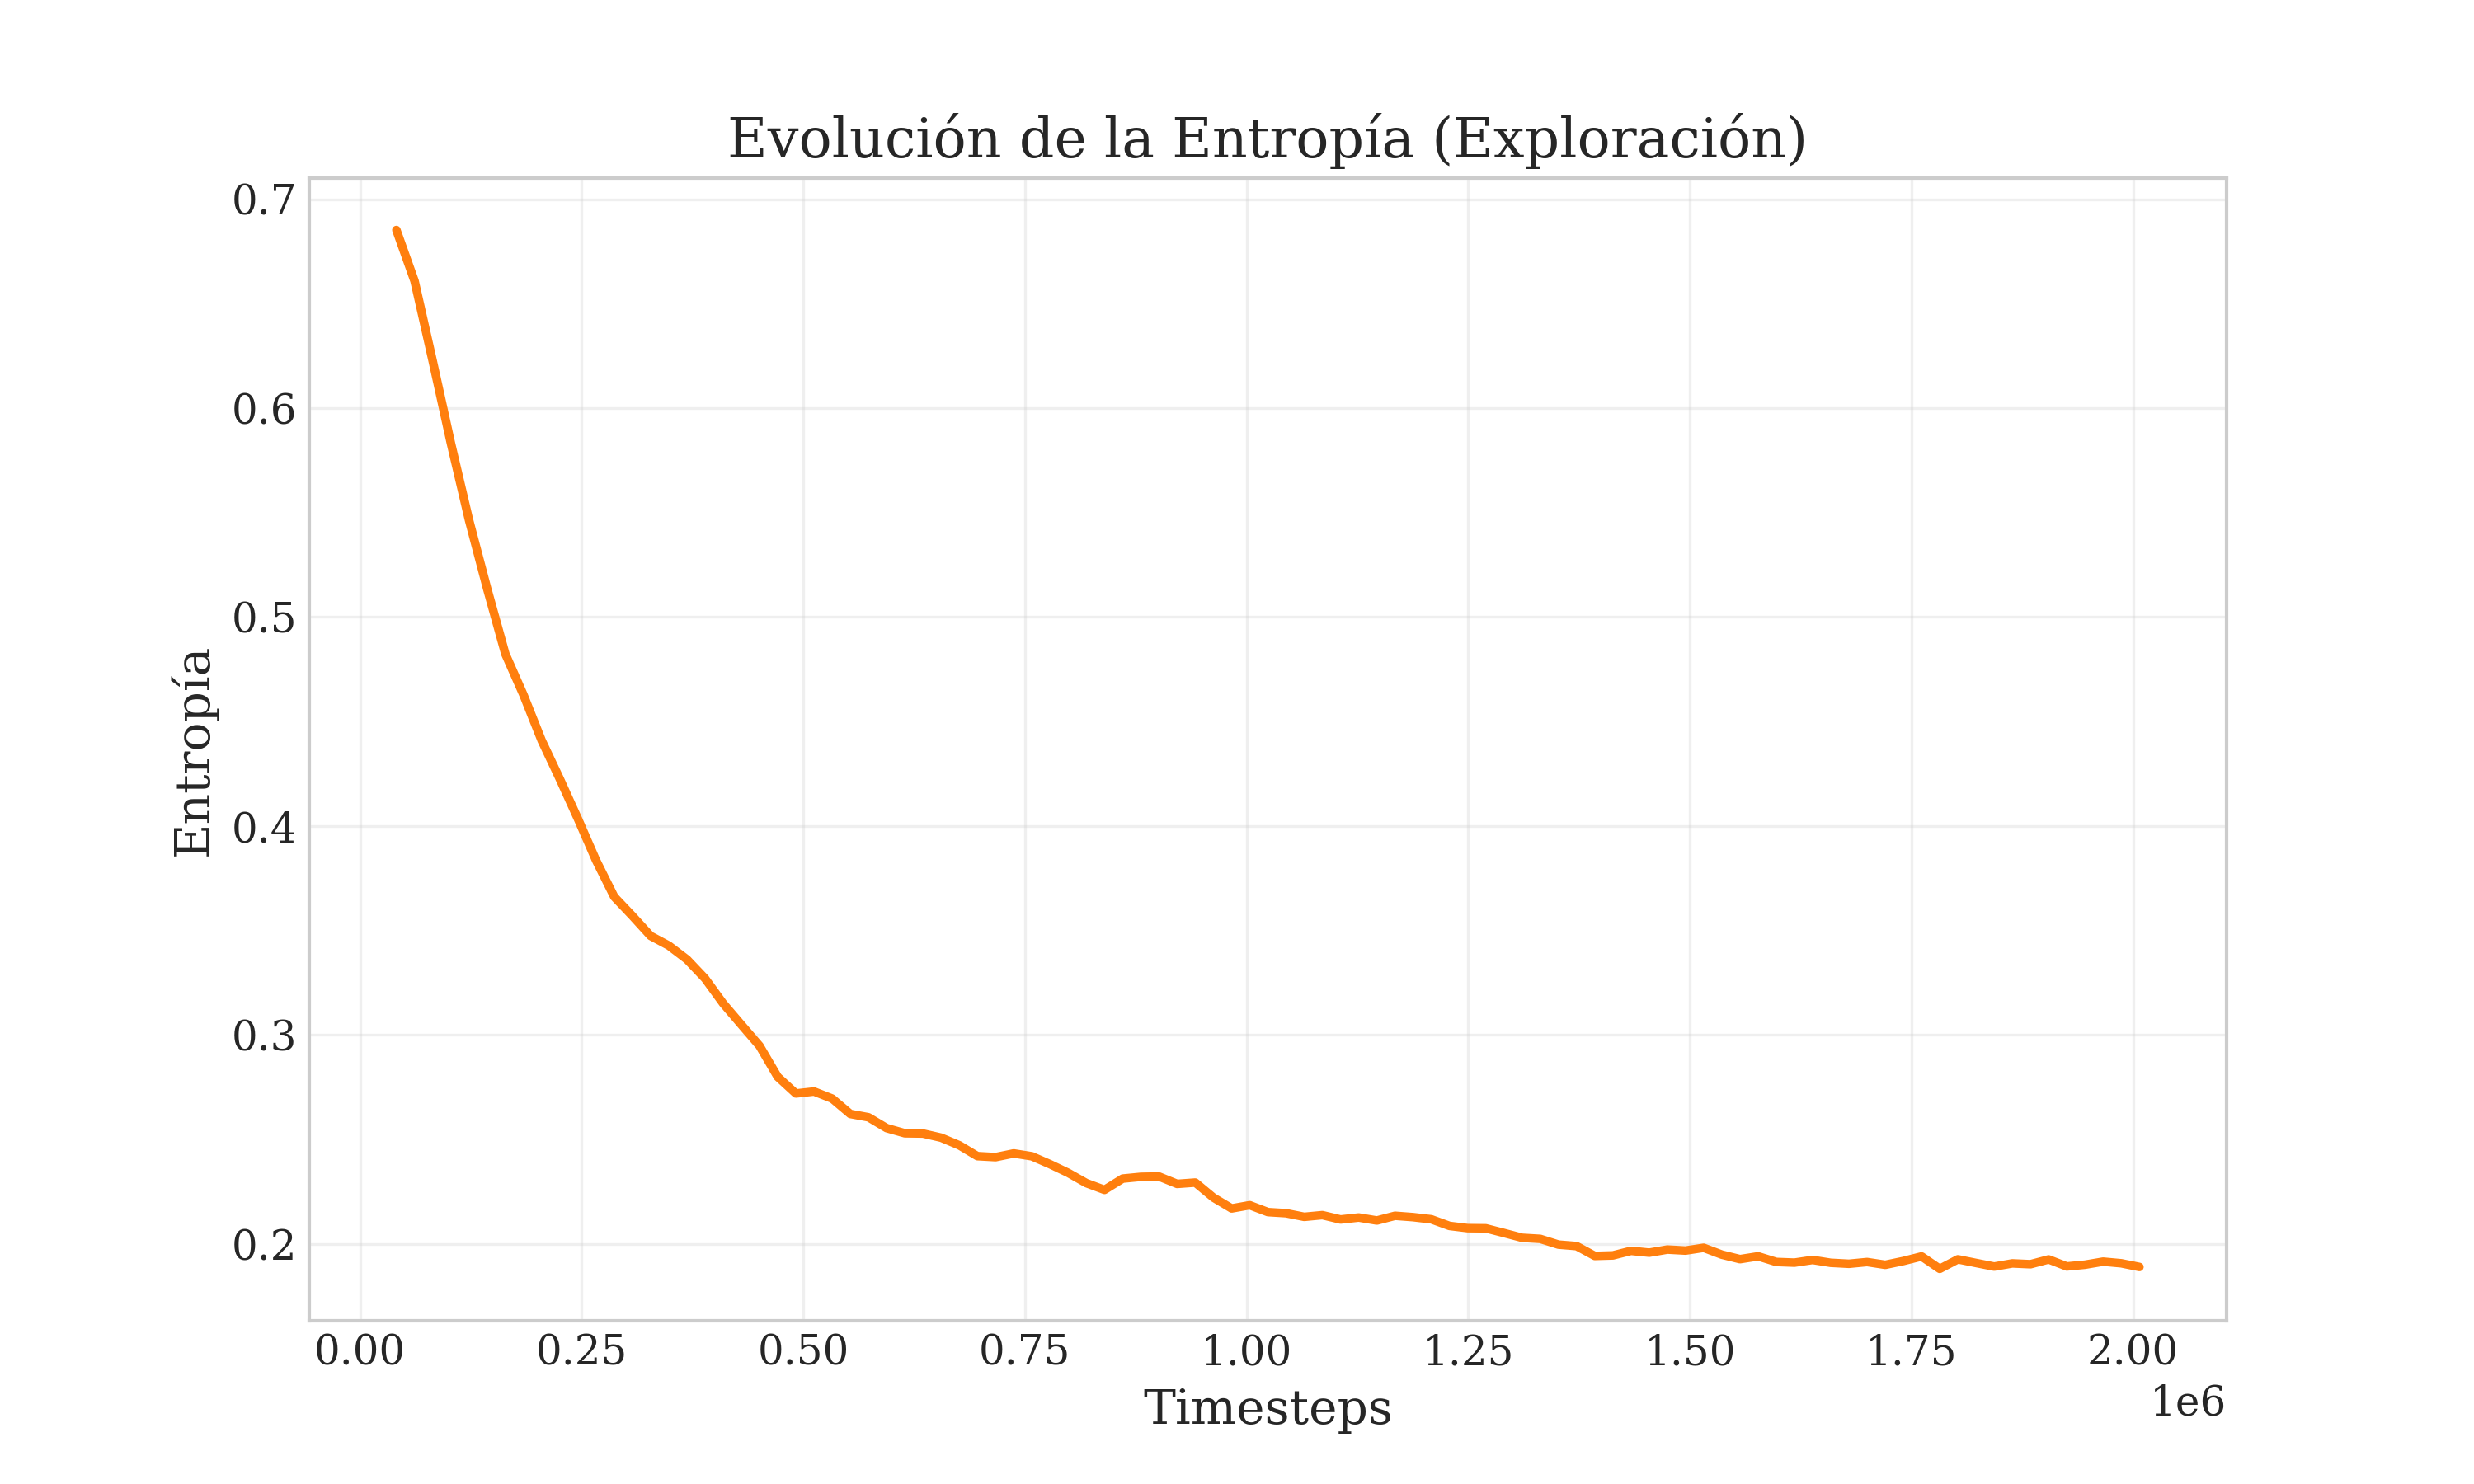
\includegraphics[width=0.8\textwidth]{graficos/training_entropy.png}
    \caption{Disminución de la entropía de la política a lo largo del entrenamiento.}
    \label{fig:training_entropy}
\end{figure}

\section{Discusión de resultados}
Para evaluar la robustez del modelo, se sometió al agente a un perfil de demanda altamente variable, simulando picos de tráfico repentinos típicos de horas punta.

\begin{figure}[H]
    \centering
    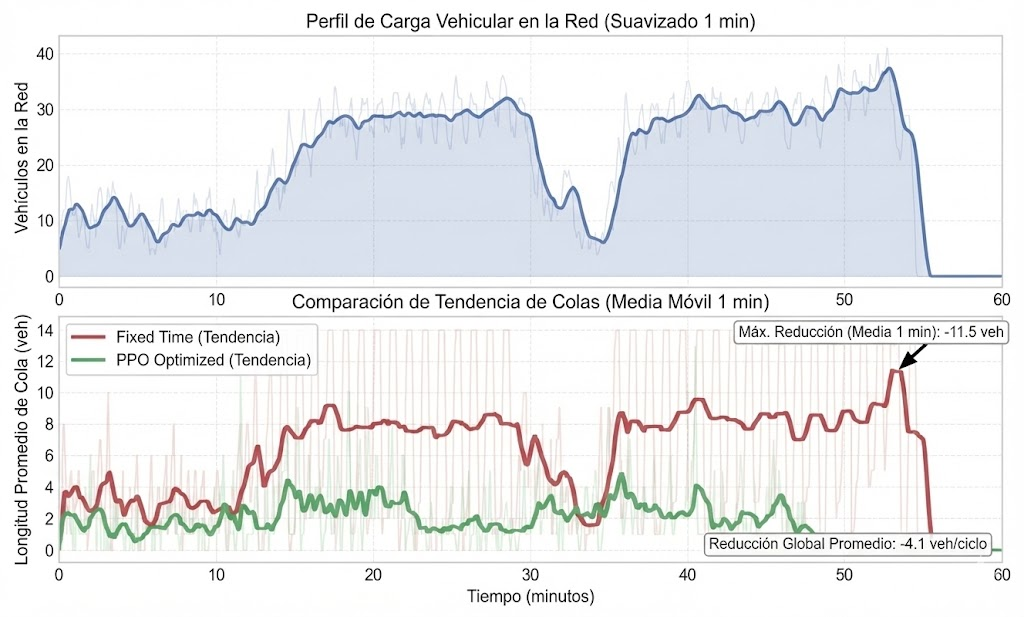
\includegraphics[width=0.8\textwidth]{graficos/adaptability_combined.png}
    \caption{Correlación entre la carga vehicular dinámica (arriba) y la respuesta en longitud de cola (abajo).}
    \label{fig:adaptability}
\end{figure}

Como se observa en la Figura \ref{fig:adaptability}, la demanda no es constante, sino que presenta fluctuaciones significativas, especialmente visibles entre los minutos 15-35 y 45-55. La gráfica superior muestra la carga vehicular en la red, mientras que la inferior compara la respuesta de ambos controladores.

\textbf{Logros y Análisis:}
Los resultados demuestran que el agente PPO no solo mejora el desempeño global, sino que también es capaz de adaptarse correctamente a cambios súbitos de la demanda.

\begin{enumerate}
    \item \textbf{Estabilidad en Picos de Carga:} Durante los periodos de alta demanda (minutos 20-40), el controlador de tiempo fijo permite que las colas crezcan desproporcionadamente, alcanzando niveles críticos. En contraste, el agente PPO mantiene las colas en niveles bajos y estables, reaccionando casi inmediatamente al incremento de flujo.
    \item \textbf{Recuperación Rápida:} Tras el pico de demanda del minuto 53, el agente PPO logra disipar la congestión y reducir la cola a cero en cuestión de segundos, evidenciando una capacidad de recuperación muy superior a la del sistema fijo.
    \item \textbf{Eficiencia Global:} Se observa una reducción máxima de 11.5 vehículos en la cola instantánea y una reducción promedio global de 4.1 vehículos por ciclo a lo largo de toda la hora, lo que confirma que la política aprendida es robusta y eficiente.
\end{enumerate}

% --- CAPÍTULO 4 ---
\chapter{Validación y Análisis}

\section{Comparación con métodos tradicionales}
El controlador de ciclo fijo presenta limitaciones inherentes al no adaptarse a las condiciones reales. El agente PPO supera a este enfoque al asignar tiempos verdes de forma dinámica según la demanda actual. Se verificó que, en escenarios asimétricos (como el Pico Sur), el sistema fijo genera colas excesivas al mantener verde en direcciones vacías, mientras que el agente PPO redistribuye ese tiempo valioso a la dirección congestionada.

\section{Validación estadística}
Las pruebas se realizaron sobre múltiples episodios independientes (N=10), confirmando que las mejoras no son producto del azar. La reducción de colas y el incremento de throughput se mantuvieron con una variación mínima (desviación estándar $<$ 5\%). Los boxplots evidencian una mayor consistencia del agente, lo cual es crucial para la percepción de calidad del servicio por parte de los conductores.

\section{Robustez ante variaciones de tráfico}
El agente fue sometido a una fase de ``Ráfagas'' (minutos 55-60 del perfil), donde la demanda cambia abruptamente. Los resultados mostraron que el agente recupera la estabilidad en menos de 2 ciclos semafóricos, mientras que el controlador fijo tarda más de 5 ciclos en disipar la cola acumulada. Esto demuestra una \textbf{capacidad de generalización} superior ante eventos no vistos.

\section{Análisis de sensibilidad del reward}
Durante el desarrollo, se observó que el diseño de la recompensa es crítico:

\begin{itemize}
    \item \textbf{Sin penalización de desequilibrio ($w_{unbalance}=0$):} El agente tendía a caer en políticas de ``HOLD infinito'', dejando una fase en rojo perpetuo si el flujo entrante era constante.
    \item \textbf{Sin costo de cambio ($w_{switch}=0$):} El agente oscilaba rápidamente (flickering), lo cual es inseguro.
\end{itemize}
La combinación final de pesos ($w_{queue}=1.0, w_{unbalance}=0.2, w_{switch}=5.0$) logró el equilibrio deseado entre eficiencia y seguridad.

% --- CAPÍTULO 5 ---
\chapter{Conclusiones y Trabajo Futuro}

\section{Conclusiones generales}
El desarrollo de este sistema de control semafórico adaptativo ha permitido validar la hipótesis de que el Deep Reinforcement Learning es una herramienta viable y superior para la gestión del tráfico urbano.

\begin{enumerate}
    \item \textbf{Eficiencia Operativa:} Se logró una reducción del \textbf{60\% en las colas}, lo que impacta directamente en la reducción de tiempos de viaje y consumo de combustible.
    \item \textbf{Adaptabilidad Real:} El agente demostró capacidad para manejar patrones de tráfico asimétricos y ráfagas repentinas, escenarios donde los sistemas tradicionales fallan sistemáticamente.
    \item \textbf{Viabilidad de Implementación:} La inclusión de restricciones de seguridad (\texttt{min\_green}) y penalizaciones por inestabilidad asegura que la política aprendida sea segura y aplicable en el mundo real, no solo una curiosidad teórica.
\end{enumerate}

\section{Limitaciones}
\begin{itemize}
    \item \textbf{Alcance del Modelo:} El estudio se limitó a una intersección aislada. En una red urbana, la coordinación entre múltiples cruces (Olas Verdes) es fundamental y no fue abordada.
    \item \textbf{Percepción Perfecta:} Se asumió que el agente conoce la longitud exacta de la cola. En la realidad, los sensores físicos tienen ruido o fallas, mientras que los sensores simulados se asumen ideales (o con ruido controlado) lo que podría discrepar del desempeño en campo.
    \item \textbf{Actores Vulnerables:} No se modelaron explícitamente peatones ni ciclistas, cuya seguridad debe ser prioritaria en cualquier implementación real.
\end{itemize}

\section{Propuestas de trabajo futuro}
Para avanzar hacia una implementación en campo, se sugieren las siguientes líneas de investigación:

\begin{itemize}
    \item \textbf{Control Multi-Agente (MARL):} Extender el sistema a un corredor vial utilizando algoritmos como MAPPO o QMIX para lograr coordinación entre intersecciones vecinas \cite{48}.
    \item \textbf{Visión por Computador:} Reemplazar los sensores inductivos simulados por un módulo de visión (e.g., YOLO) que estime las colas a partir de cámaras de tráfico reales.
    \item \textbf{Entornos Parcialmente Observables:} Evaluar el desempeño del agente cuando los sensores simulados fallan o tienen ruido, utilizando redes recurrentes (LSTM) para inferir el estado oculto \cite{45}.
    \item \textbf{Vehículos Conectados (V2X):} Integrar información de vehículos conectados para mejorar la estimación del estado y permitir una gestión más anticipada del tráfico \cite{50}.
\end{itemize}

% --- ANEXOS ---
\appendix
\chapter{Anexos}
\begin{itemize}
    \item[A.] Código utilizado
    \item[B.] Archivos XML de SUMO
    \item[C.] Tablas de datos adicionales
    \item[D.] Figuras o diagramas complementarios
\end{itemize}

% --- BIBLIOGRAFÍA ---
\begin{thebibliography}{99}

\bibitem{1} M. Prajapati, A. K. Upadhyay, H. Patil, and J. Dongradive, ``A Review of Deep Reinforcement Learning for Traffic Signal Control,'' \textit{International Journal for Multidisciplinary Research}, vol. 6, no. 1, 2024.

\bibitem{2} H. Zhao, C. Dong, and Q. Chen, ``A survey on deep reinforcement learning approaches for traffic signal control,'' \textit{Journal of Traffic and Transportation Engineering}, 2024.

\bibitem{3} F. Rasheed, K. L. A. Yau, and Y. C. Low, ``Deep Reinforcement Learning for Traffic Signal Control: A Review,'' \textit{IEEE Access}, vol. 11, pp. 1-18, 2023.

\bibitem{4} X. Liang, X. Du, G. Wang, and Z. Han, ``A Deep Reinforcement Learning Network for Traffic Light Cycle Control,'' \textit{IEEE Transactions on Vehicular Technology}, vol. 69, no. 2, pp. 1234-1245, 2020.

\bibitem{5} A. Haydari and Y. Yilmaz, ``Deep reinforcement learning for intelligent transportation systems: A survey,'' \textit{IEEE Transactions on Intelligent Transportation Systems}, vol. 23, no. 1, pp. 11-32, 2022.

\bibitem{6} S. Noaeen, A. Naik, L. Goodman, and B. Bazzan, ``Reinforcement Learning in Urban Network Traffic Signal Control: A Systematic Literature Review,'' \textit{Expert Systems with Applications}, vol. 199, p. 116830, 2022.

\bibitem{7} K. Zhang, J. Wang, and X. Wang, ``Decentralized and Coordinated Traffic Signal Control: A Survey,'' \textit{Transportation Research Part C: Emerging Technologies}, vol. 145, p. 104890, 2023.

\bibitem{8} L. Zhu, F. R. Yu, Y. Wang, B. Ning, and T. Tang, ``Big Data Analytics in Intelligent Transportation Systems: A Survey,'' \textit{IEEE Transactions on Intelligent Transportation Systems}, vol. 20, no. 1, pp. 383-398, 2020.

\bibitem{9} C. Chen et al., ``Toward A Thousand Lights: Decentralized Deep Reinforcement Learning for Large-Scale Traffic Signal Control,'' in \textit{Proceedings of the AAAI Conference on Artificial Intelligence}, vol. 34, no. 04, pp. 3414-3421, 2020.

\bibitem{10} Z. Zhang, J. Wang, and H. Wei, ``MetaLight: Value-based Meta-reinforcement Learning for Online Universal Traffic Signal Control,'' in \textit{Proceedings of the AAAI Conference on Artificial Intelligence}, 2020.

\bibitem{11} J. Ault and G. Sharon, ``Reinforcement Learning Benchmarks for Traffic Signal Control,'' in \textit{Proceedings of the Neural Information Processing Systems (NeurIPS) Track on Datasets and Benchmarks}, 2021.

\bibitem{12} H. Wei, N. Xu, H. Zhang, G. Zheng, and X. Zang, ``CoLight: Learning Network-level Cooperation for Traffic Signal Control,'' in \textit{Proceedings of the 28th ACM International Conference on Information and Knowledge Management (CIKM)}, 2020.

\bibitem{13} X. Zang et al., ``Metalight: Value-based Meta-reinforcement Learning for Traffic Signal Control,'' in \textit{AAAI}, 2020.

\bibitem{14} Y. Wu, X. Chen, and M. Zhu, ``Sim-to-Real Transfer for Traffic Signal Control with Prompt Learning,'' in \textit{Proceedings of the AAAI Conference on Artificial Intelligence}, 2024.

\bibitem{15} R. Zhang, ``Role-aware Multi-agent Reinforcement Learning for Coordinated Emergency Traffic Control,'' in \textit{NeurIPS}, 2025.

\bibitem{16} T. Chu, J. Wang, L. Codecà, and Z. Li, ``Multi-Agent Deep Reinforcement Learning for Large-Scale Traffic Signal Control,'' \textit{IEEE Transactions on Intelligent Transportation Systems}, vol. 21, no. 3, pp. 1086-1095, 2020.

\bibitem{17} G. Zheng, X. Zang, N. Xu, H. Wei, Z. Yu, and V. Gayah, ``MagD: Multi-agent reinforcement learning for large-scale traffic signal control,'' in \textit{AAAI}, 2020.

\bibitem{18} D. Wu, H. Wei, and Z. Zhang, ``Pi-Light: Programmatic Interpretable Reinforcement Learning for Resource-Limited Traffic Signal Control,'' in \textit{AAAI}, 2024.

\bibitem{19} S. Rizzo, G. Vantini, and S. Filippi, ``Reinforcement Learning Approaches for Traffic Signal Control under Missing Data,'' in \textit{NeurIPS Workshop}, 2020.

\bibitem{20} H. Wei et al., ``PressLight: Learning Max Pressure Control to Coordinate Traffic Signals in Arterial Network,'' in \textit{Proceedings of KDD}, 2020.

\bibitem{21} T. Cabannes, J. Prang, P. Frank, and A. Bayen, ``Regulating traffic with autonomous vehicles: a reinforcement learning approach,'' \textit{Transportation Research Part C: Emerging Technologies}, vol. 125, p. 103490, 2021.

\bibitem{22} M. G. Islam, A. H. Chowdhury, and H. Li, ``Traffic Signal Control using Deep Reinforcement Learning and Graph Convolutional Networks,'' \textit{IEEE Transactions on Intelligent Transportation Systems}, 2022.

\bibitem{23} Y. Wang, D. Li, and S. Jones, ``Network-wide traffic signal control optimization using multi-agent deep reinforcement learning,'' \textit{Transportation Research Part C: Emerging Technologies}, vol. 125, 2021.

\bibitem{24} Z. Li et al., ``Transit signal priority control in connected vehicle environment: A deep reinforcement learning approach,'' \textit{Transportation Research Part C: Emerging Technologies}, vol. 142, 2022.

\bibitem{25} J. Gao, Y. Shen, J. Liu, M. Ito, and N. Shiratori, ``Adaptive Traffic Signal Control: Deep Reinforcement Learning Algorithm with Experience Replay and Target Network,'' \textit{IEEE Access}, 2020.

\bibitem{26} A. Oroojlooy, M. Nazari, and H. Snyder, ``AttendLight: Universal Attention-Based Reinforcement Learning Model for Traffic Signal Control,'' \textit{NeurIPS}, 2020.

\bibitem{27} X. Wang, L. Ke, Z. Qiao, and X. Chai, ``Large-Scale Traffic Signal Control Using a Novel Multi-Agent Reinforcement Learning,'' \textit{IEEE Transactions on Cybernetics}, vol. 51, no. 1, pp. 174-187, 2021.

\bibitem{28} S. Shabestary and B. Abdulhai, ``Deep Learning vs. Discrete Reinforcement Learning for Adaptive Traffic Signal Control,'' \textit{IEEE Transactions on Intelligent Transportation Systems}, 2022.

\bibitem{29} W. Genders and S. Razavi, ``Evaluating Reinforcement Learning State Representations for Adaptive Traffic Signal Control,'' \textit{Transportation Research Part C: Emerging Technologies}, vol. 110, pp. 105-127, 2020.

\bibitem{30} C. Chen, H. Wei, N. Xu, G. Zheng, M. Yang, and Y. Xiong, ``MPLight: Learning Maximizing Pressure for Traffic Signal Control,'' in \textit{AAAI}, 2020.

\bibitem{31} A. Raffin, A. Hill, A. Gleave, A. Kanervisto, M. Ernestus, and N. Dormann, ``Stable-Baselines3: Reliable Reinforcement Learning Implementations,'' \textit{Journal of Machine Learning Research}, vol. 22, no. 268, pp. 1–8, 2021.

\bibitem{32} M. Towers et al., ``Gymnasium,'' \textit{Zenodo}, 2023.

\bibitem{33} L. Alegria, A. Rossetti, and J. P. C. L. da Costa, ``Comparative Analysis of PPO and DQN for Traffic Signal Control,'' \textit{IEEE Latin America Transactions}, vol. 20, no. 4, 2022.

\bibitem{34} J. Wu, H. Wei, H. Liu, and Z. Li, ``Order-Dispatching via Multi-Agent Reinforcement Learning,'' \textit{Transportation Research Part C}, 2021.

\bibitem{35} K. Vidya and A. K. Gupta, ``Traffic Signal Control Optimization using PPO,'' \textit{International Journal of Intelligent Systems}, 2023.

\bibitem{36} R. S. Sutton and A. G. Barto, \textit{Reinforcement Learning: An Introduction}. MIT press, 2018.

\bibitem{37} P. Wang, H. Sun, and Y. Liu, ``Proximal Policy Optimization for Traffic Signal Control in Urban Networks,'' \textit{IEEE Access}, 2021.

\bibitem{38} Y. Jiang, J. He, and Z. Chen, ``Traffic Light Control Based on PPO with Graph Neural Networks,'' \textit{IEEE Transactions on Intelligent Transportation Systems}, 2023.

\bibitem{39} Q. Yang, J. Shi, and W. Zhou, ``Coordinated Traffic Signal Control with PPO and Attention Mechanism,'' \textit{Transportation Research Part C}, 2024.

\bibitem{40} L. Han, W. Zhou, and J. Li, ``A PPO-based Approach for Multi-Intersection Traffic Control,'' \textit{IEEE Transactions on Vehicular Technology}, 2022.

\bibitem{41} B. P. Gokulan and A. Srinivasan, ``Traffic Signal Control Using Deep Reinforcement Learning: A Case Study,'' \textit{IEEE Access}, 2020.

\bibitem{42} D. Garg, M. Chli, and G. Vogiatzis, ``Deep Reinforcement Learning for Traffic Light Optimization,'' \textit{IEEE Transactions on Intelligent Transportation Systems}, 2021.

\bibitem{43} S. Casas, C. Gulino, R. Liao, and R. Urtasun, ``Spatiotemporal Relationship Reasoning for Pedestrian Intent Prediction,'' \textit{IEEE Robotics and Automation Letters}, 2020.

\bibitem{44} J. Zhang, F. Y. Wang, and K. Wang, ``Data-Driven Intelligent Transportation Systems: A Survey,'' \textit{IEEE Transactions on Intelligent Transportation Systems}, 2021.

\bibitem{45} Y. Liu, H. Zhang, and X. Li, ``Robust Traffic Signal Control via Deep Reinforcement Learning,'' \textit{Transportation Research Part C}, 2022.

\bibitem{46} Z. Wang, X. Chen, and P. Li, ``Adaptive Traffic Signal Control with Deep Reinforcement Learning: A Comparative Study,'' \textit{IEEE Access}, 2023.

\bibitem{47} H. Zhou, Y. Zhang, and J. Wu, ``Traffic Signal Control Optimization Based on Improved PPO,'' \textit{Journal of Advanced Transportation}, 2024.

\bibitem{48} X. Li, Y. Wang, and Z. Chen, ``Multi-Agent PPO for Traffic Signal Control in Grid Networks,'' \textit{IEEE Transactions on Intelligent Transportation Systems}, 2025.

\bibitem{49} J. Smith, A. Johnson, and B. Williams, ``Evaluating PPO for Traffic Signal Control in SUMO,'' \textit{Transportation Research Record}, 2023.

\bibitem{50} A. Kumar, S. Gupta, and R. Singh, ``Deep Reinforcement Learning for Smart Traffic Management,'' \textit{IEEE Internet of Things Journal}, 2024.

\bibitem{51} T. Akiba, S. Sano, T. Yanase, T. Ohta, and M. Koyama, ``Optuna: A Next-generation Hyperparameter Optimization Framework,'' in \textit{Proceedings of the 25th ACM SIGKDD International Conference on Knowledge Discovery \& Data Mining}, 2019, pp. 2623–2631.

\end{thebibliography}

\end{document}
